% ==================================================
% ==================================================
\chapter{Experiments}
\label{experiments}
This chapter outlines the experiments conducted to evaluate the performance of the LR and four presented CNN models on both the smaller and larger datasets. The experiments include testing different numbers of training samples to evaluate their impact on model performance and optimizing the number of input cortical neurons to optimize the models' number of parameters and identify the most important neurons. Additionally, we explore various loss functions to determine the most suitable for our problem. The main goal of these experiments is to identify the best model for accurately generating stimulus images from cortical activity.

In this chapter, we begin by describing the experiments conducted on the ten-trials dataset~\ref{experiments:ten-trials}. We evaluate the models using several loss functions to find the best model. Then we examine the dataset size by training several models~\ref{experiments:ten-trials:linear-regression} and explore the effect of intrinsic noise in the cortical neurons~\ref{experiments:ten-trials:intristic-noise-limitation}.

In the next section~\ref{experiments:one-trial}, we first evaluate the models using several loss functions and show the images generated by these models~\ref{experiments:one-trial:finding-best-model}. We also examine the intermediate images, which are used internally in the architecture of two of our models~\ref{experiments:one-trial:intermediate-image}. We then use the best model to find the best loss function for training the network~\ref{experiments:one-trial:finding-best-loss}. We also evaluate the dataset size and its influence on the $L_1$ loss value in section~\ref{experiments:one-trial:number-of-samples}. The number of neurons, which are available for training is high, therefore we try to use only subsets of these neurons first in section~\ref{experiments:one-trial:number-of-inputs}, where we use a random subset from the whole population. Later in section~\ref{experiments:one-trial:population-importance}, we compare the importance of different neuron population groups, as we are provided with the information from which group (L2/3, L4, and also inhibitory or excitatory) each neuron comes.
%In the latest section~\ref{experiments:one-trial:regularization}, we present several regularization techniques, that we try.


% ==================================================
\section{Ten-trials Dataset}
\label{experiments:ten-trials}
As a toy dataset, we used the small ten-trials dataset to see how the models will perform when the number of samples is very limited. Recall that the ten-trials dataset contains $3500$ samples for training, but each stimulus in this dataset is present ten-times. As a big advantage over the second and bigger one-trial dataset, this allows us to better capture the nature of the cortical activity, which is intristicaly noisy. The evaluation of the testing dataset is present in picture~\ref{img:experiments:ten-trials:comparison} using four different loss functions -- $L_1$, MSE, SSIM, and MSSSIM.

\begin{figure}[H]\centering
  \begin{subfigure}[t]{0.45\textwidth}
    \centering
    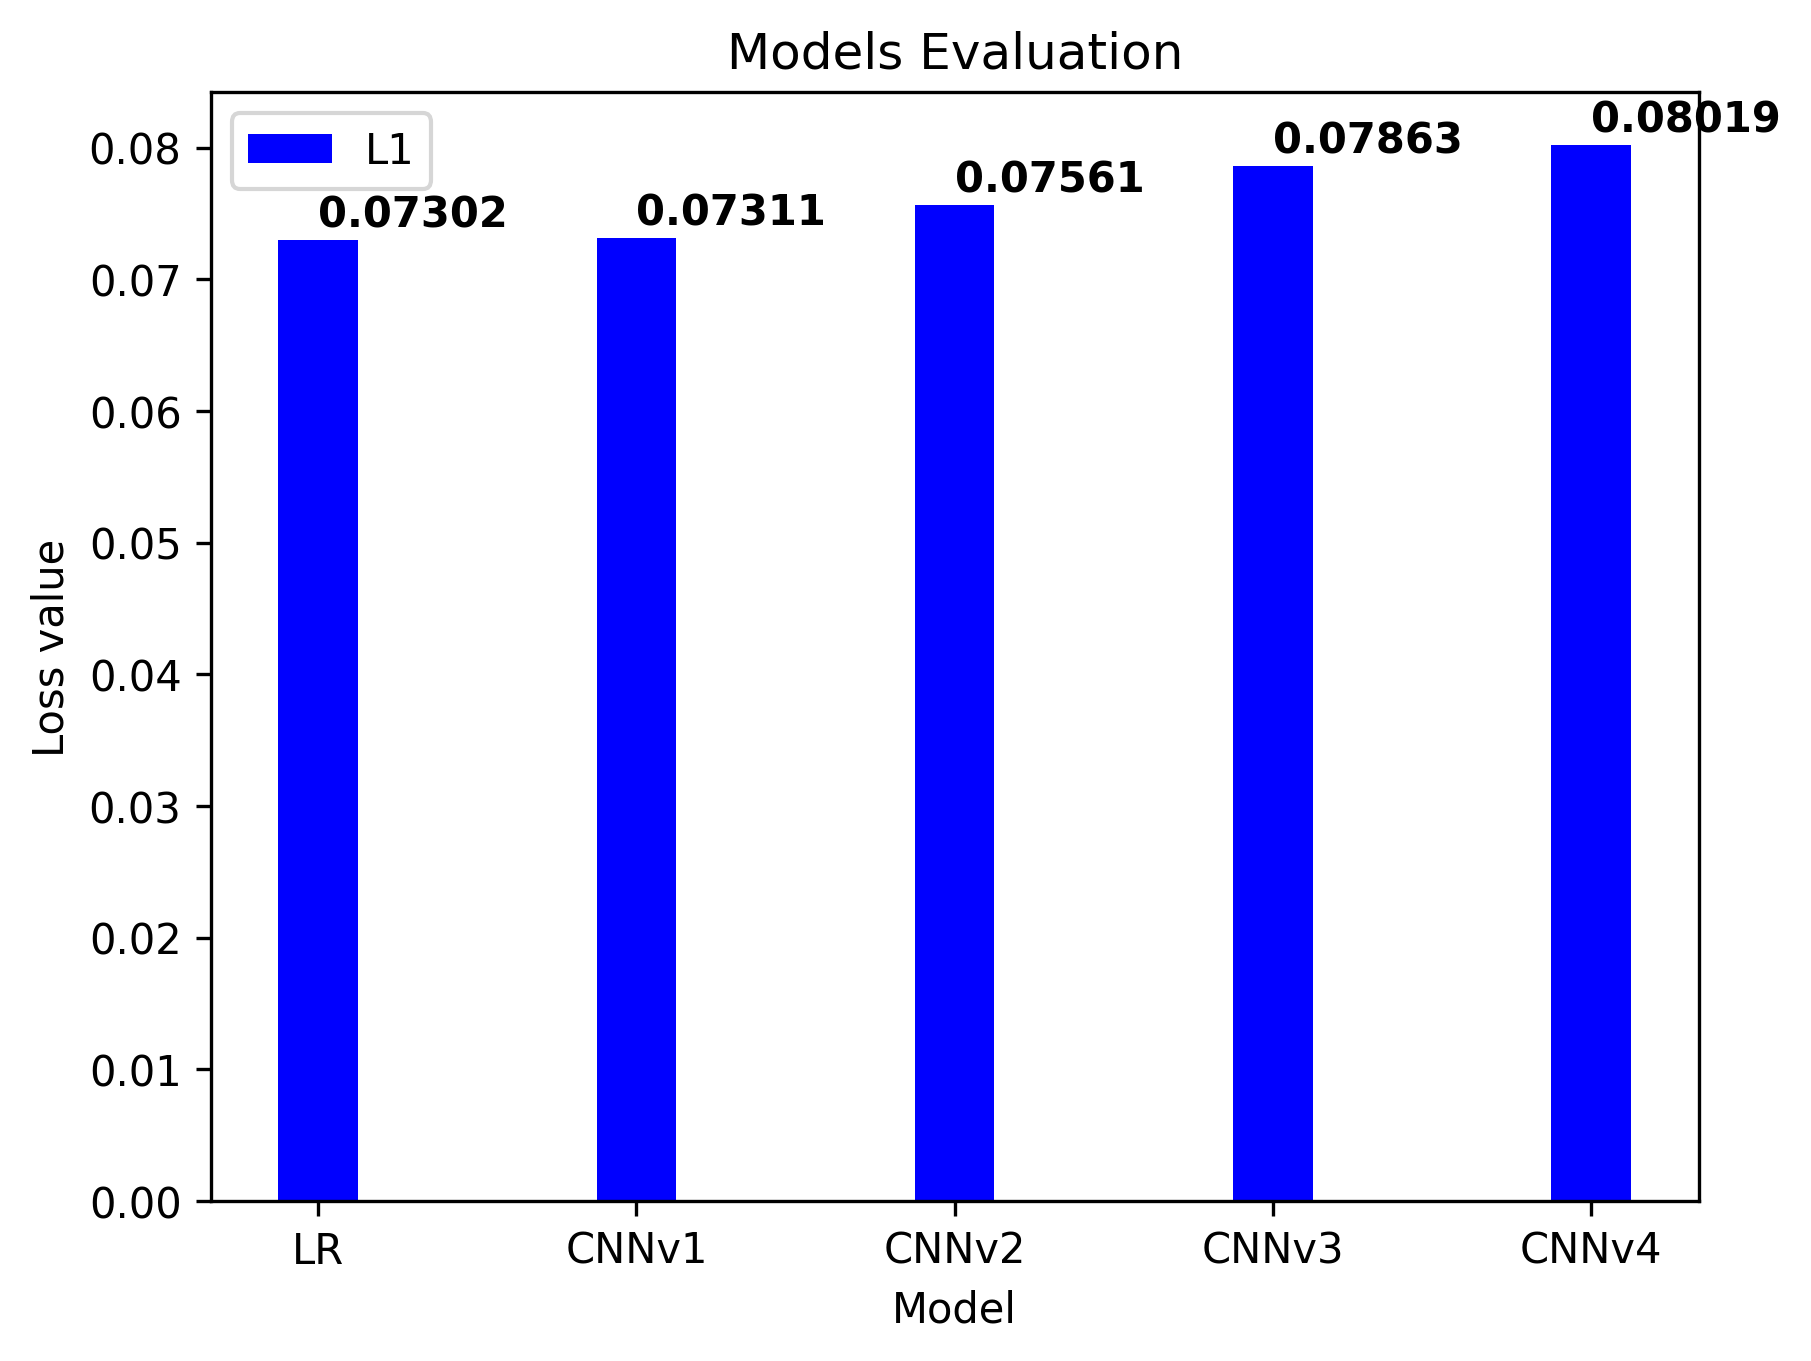
\includegraphics[width=\linewidth]{img/ten-trials/models_evaluation_ten_trials_l1.png}
    \caption{Models evaluation on $L_1$.}
  \end{subfigure}
  \begin{subfigure}[t]{0.45\textwidth}
    \centering
    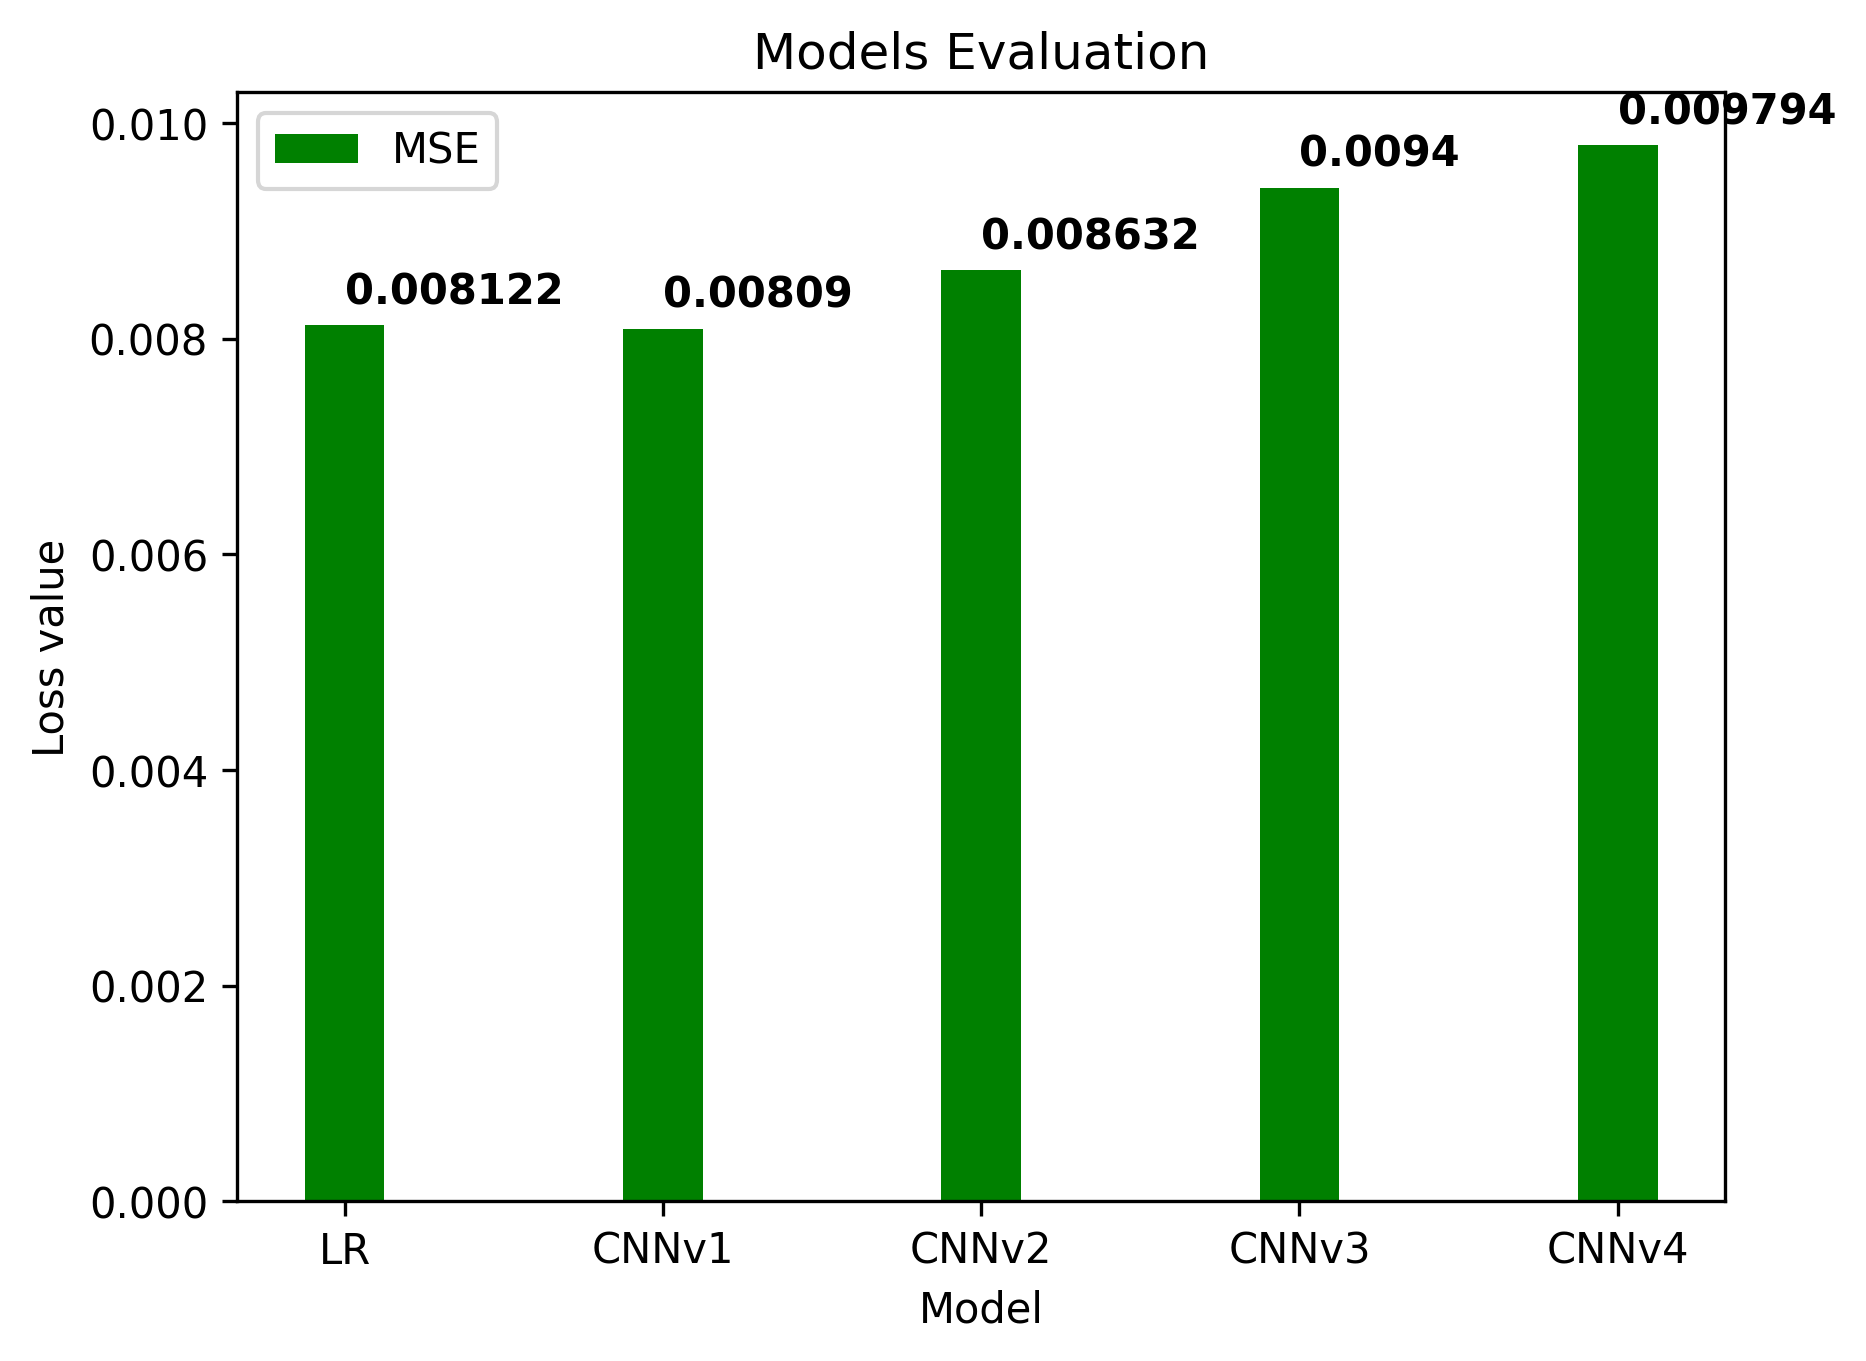
\includegraphics[width=\linewidth]{img/ten-trials/models_evaluation_ten_trials_mse.png}
    \caption{Models evaluation on MSE.}
  \end{subfigure}
  \\
  \begin{subfigure}[t]{0.45\textwidth}
    \centering
    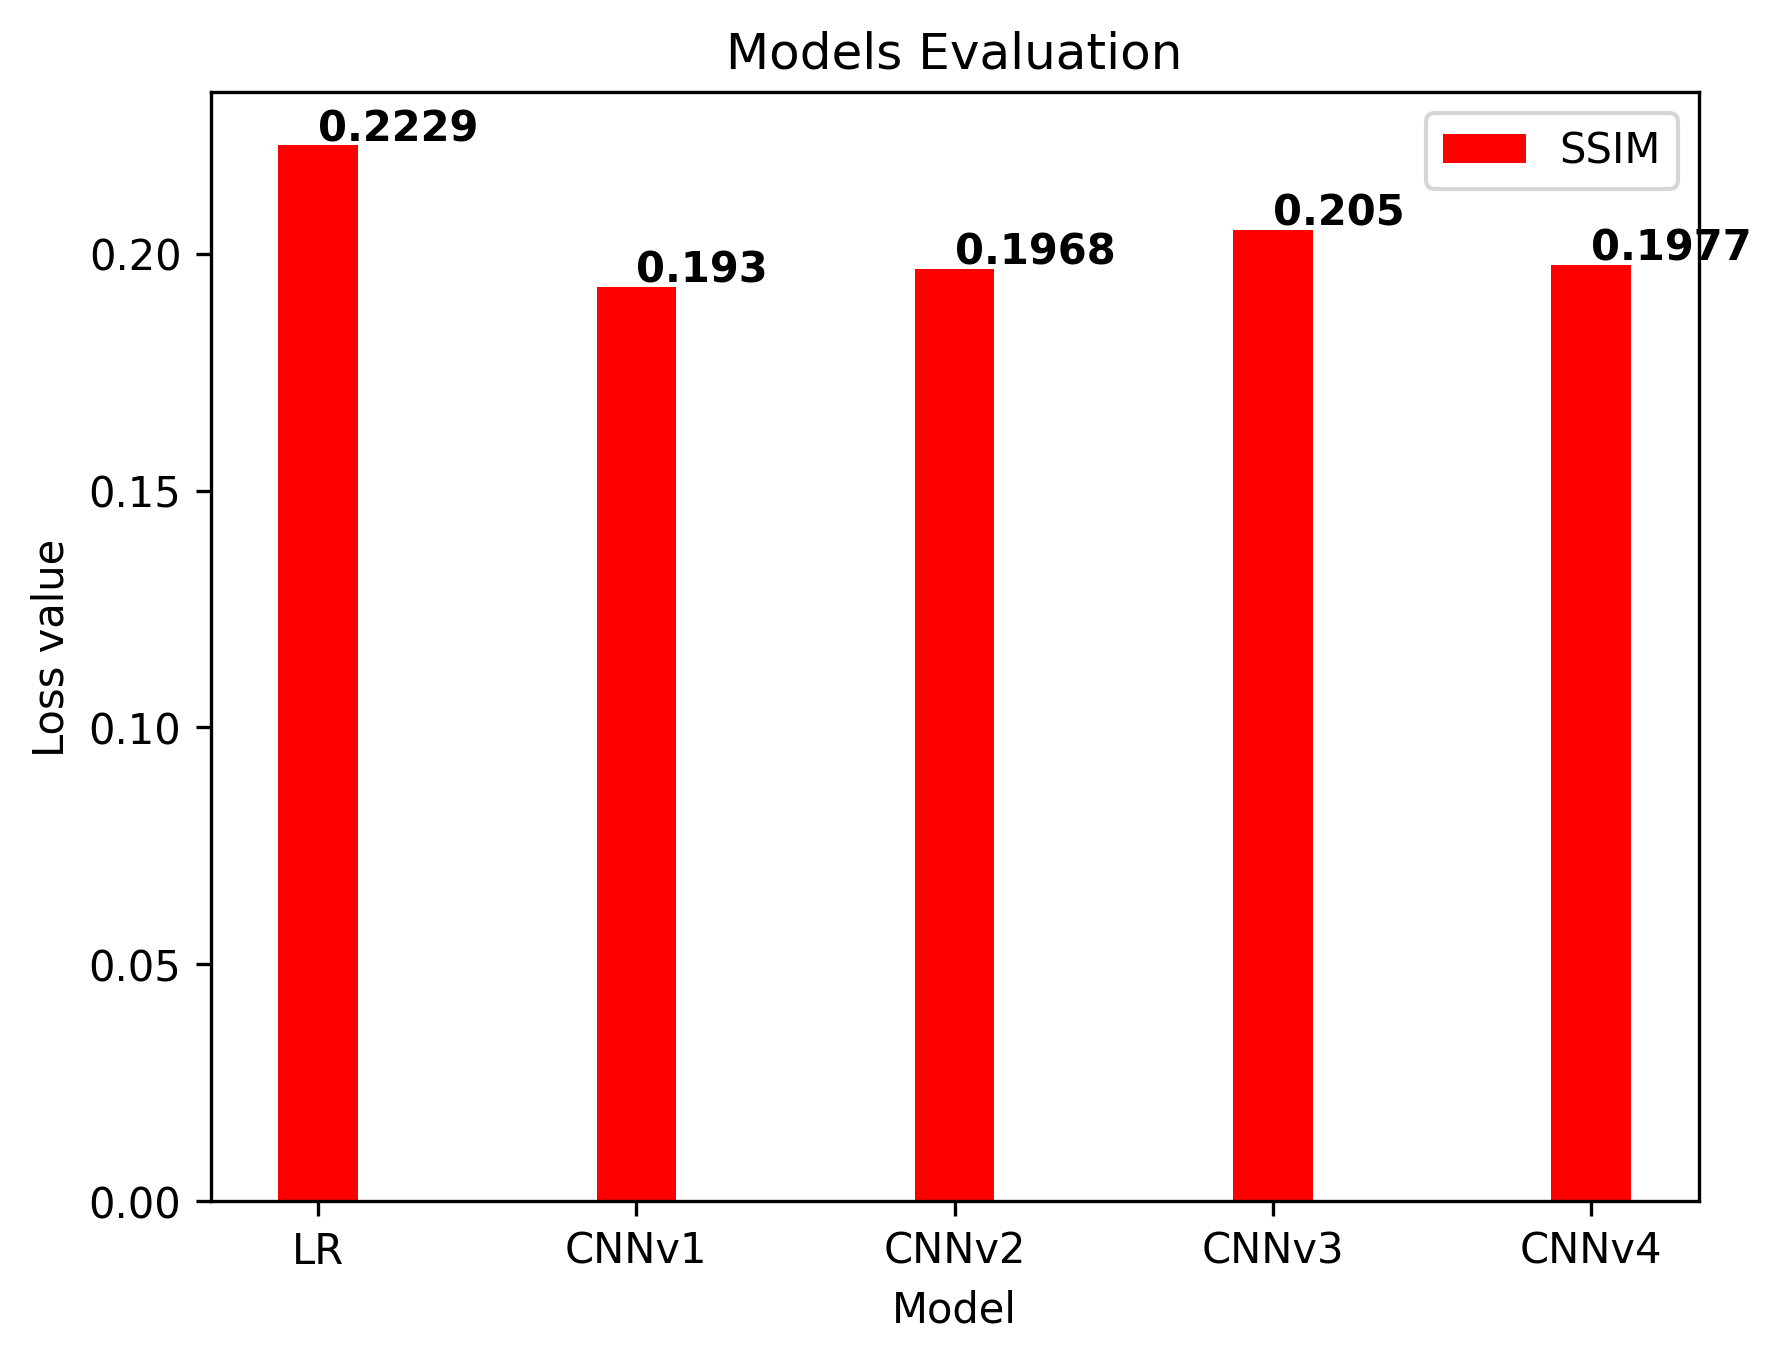
\includegraphics[width=\linewidth]{img/ten-trials/models_evaluation_ten_trials_ssim.png}
    \caption{Models evaluation on SSIM.}
  \end{subfigure}
  \begin{subfigure}[t]{0.45\textwidth}
    \centering
    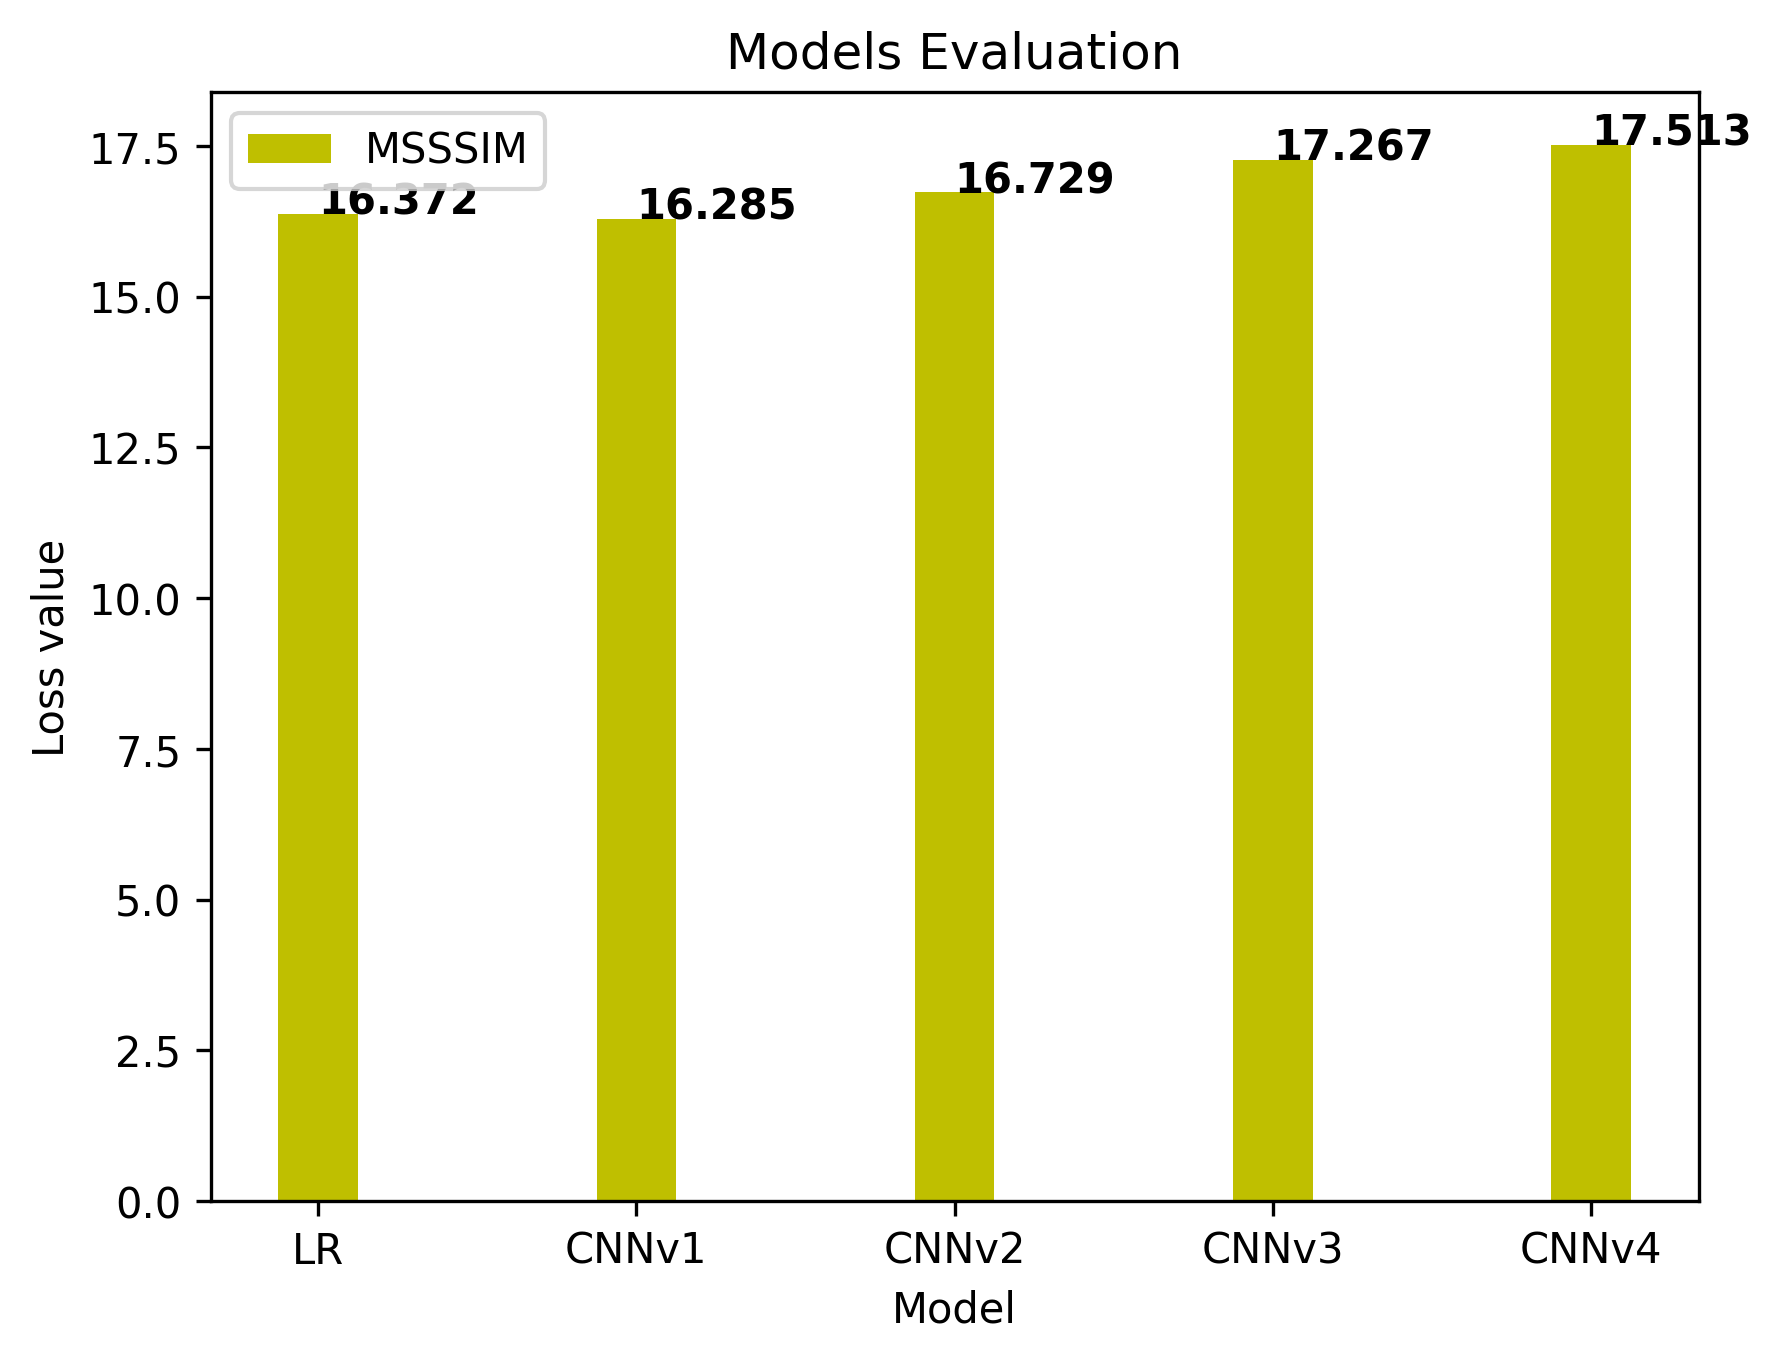
\includegraphics[width=\linewidth]{img/ten-trials/models_evaluation_ten_trials_msssim.png}
    \caption{Models evaluation on MSSSIM.}
  \end{subfigure}
  
%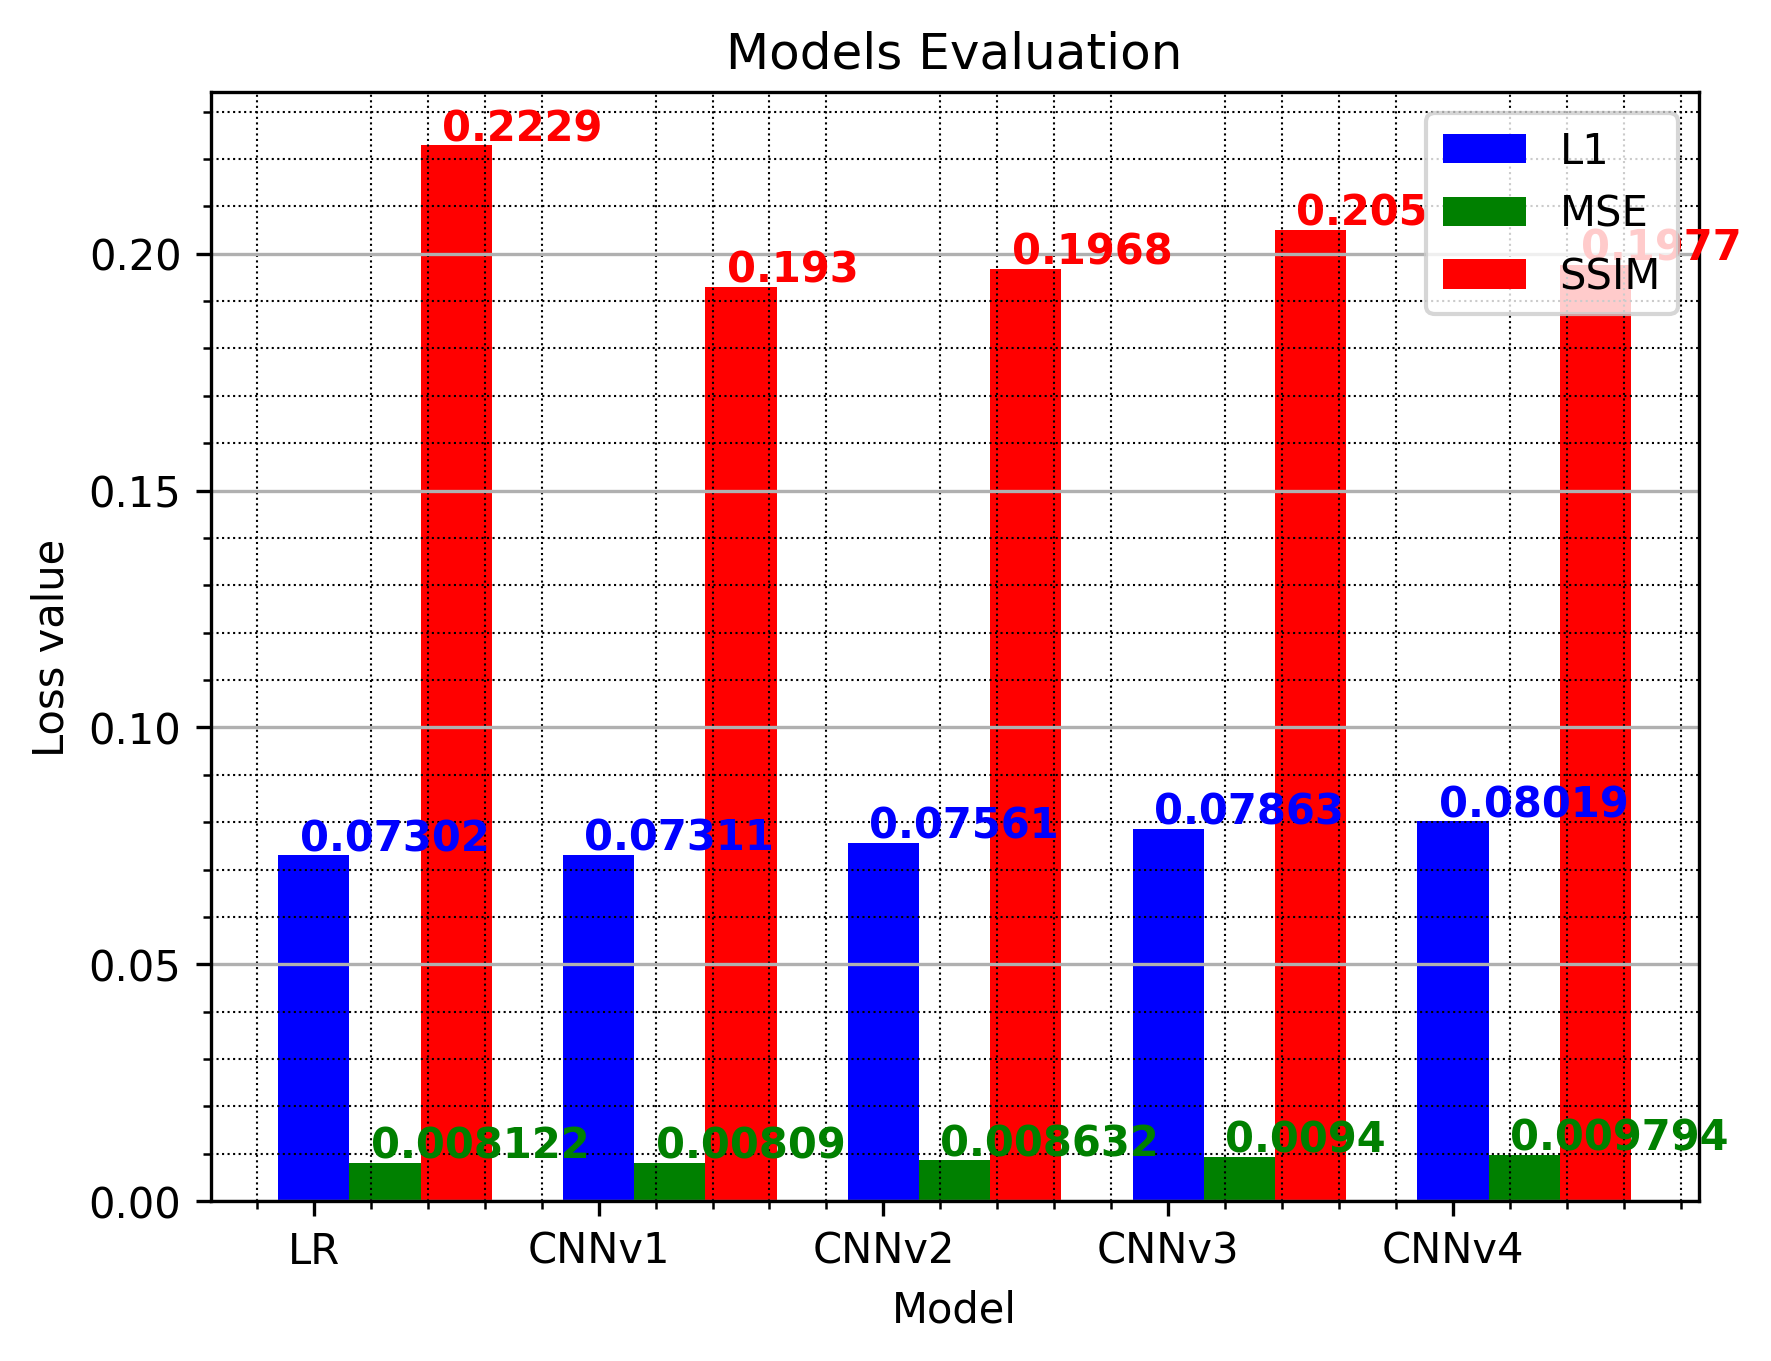
\includegraphics[width=140mm]{img/models_evaluation_ten_trials.png}
\caption{Comparison of multiple models on the same (one-trial) dataset using different loss metrics.}
\label{img:experiments:ten-trials:comparison}
\end{figure}

We can see that the linear regression (LR) and CNNv1 models compete for the lowest value in terms of $L_1$ (which is lowest for the CNNv1 model) and MSE (which is lowest for the LR model) but the values do not differ much and are comparable. The worst in terms of $L_1$ and MSE is the model CNNv4. You can compare the visual results on the testing dataset in the following image~\ref{img:experiments:ten-trials:comparison-outputs}.

\begin{figure}[H]\centering

  \begin{subfigure}[t]{0.15\textwidth}
    \centering
    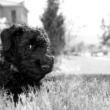
\includegraphics[width=\linewidth]{img/ten-trials/stimulus_1.png}
    %\caption{Stim. 1}
  \end{subfigure}
  \begin{subfigure}[t]{0.15\textwidth}
    \centering
    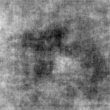
\includegraphics[width=\linewidth]{img/ten-trials/prediction_1_lr.png}
    % \caption{LR}
  \end{subfigure}
  \begin{subfigure}[t]{0.15\textwidth}
    \centering
    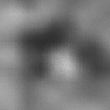
\includegraphics[width=\linewidth]{img/ten-trials/prediction_1_cnnv1.png}
    % \caption{CNNv1}
  \end{subfigure}
  \begin{subfigure}[t]{0.15\textwidth}
    \centering
    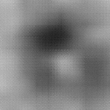
\includegraphics[width=\linewidth]{img/ten-trials/prediction_1_cnnv2.png}
    % \caption{CNNv2}
  \end{subfigure}
  \begin{subfigure}[t]{0.15\textwidth}
    \centering
    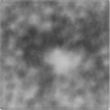
\includegraphics[width=\linewidth]{img/ten-trials/prediction_1_cnnv3.png}
    % \caption{CNNv3}
  \end{subfigure}
  \begin{subfigure}[t]{0.15\textwidth}
    \centering
    
\includegraphics[width=\linewidth]{img/ten-trials/prediction_1_cnnv4.png}
    % \caption{CNNv4}
  \end{subfigure}
  \\
    \vspace{0.1cm}
  
  \begin{subfigure}[t]{0.15\textwidth}
    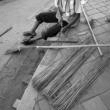
\includegraphics[width=\linewidth]{img/ten-trials/stimulus_2.png}
    \caption{Stimuli}
  \end{subfigure}
  \begin{subfigure}[t]{0.15\textwidth}
    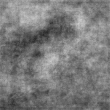
\includegraphics[width=\linewidth]{img/ten-trials/prediction_2_lr.png}
    \caption{LR}
  \end{subfigure}
  \begin{subfigure}[t]{0.15\textwidth}
    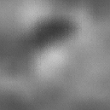
\includegraphics[width=\linewidth]{img/ten-trials/prediction_2_cnnv1.png}
    \caption{CNNv1}
  \end{subfigure}
  \begin{subfigure}[t]{0.15\textwidth}
    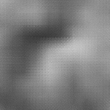
\includegraphics[width=\linewidth]{img/ten-trials/prediction_2_cnnv2.png}
    \caption{CNNv2}
  \end{subfigure}
  \begin{subfigure}[t]{0.15\textwidth}
    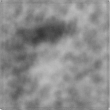
\includegraphics[width=\linewidth]{img/ten-trials/prediction_2_cnnv3.png}
    \caption{CNNv3}
  \end{subfigure}
  \begin{subfigure}[t]{0.15\textwidth}
    
\includegraphics[width=\linewidth]{img/ten-trials/prediction_2_cnnv4.png}
    \caption{CNNv4}
  \end{subfigure}
  
%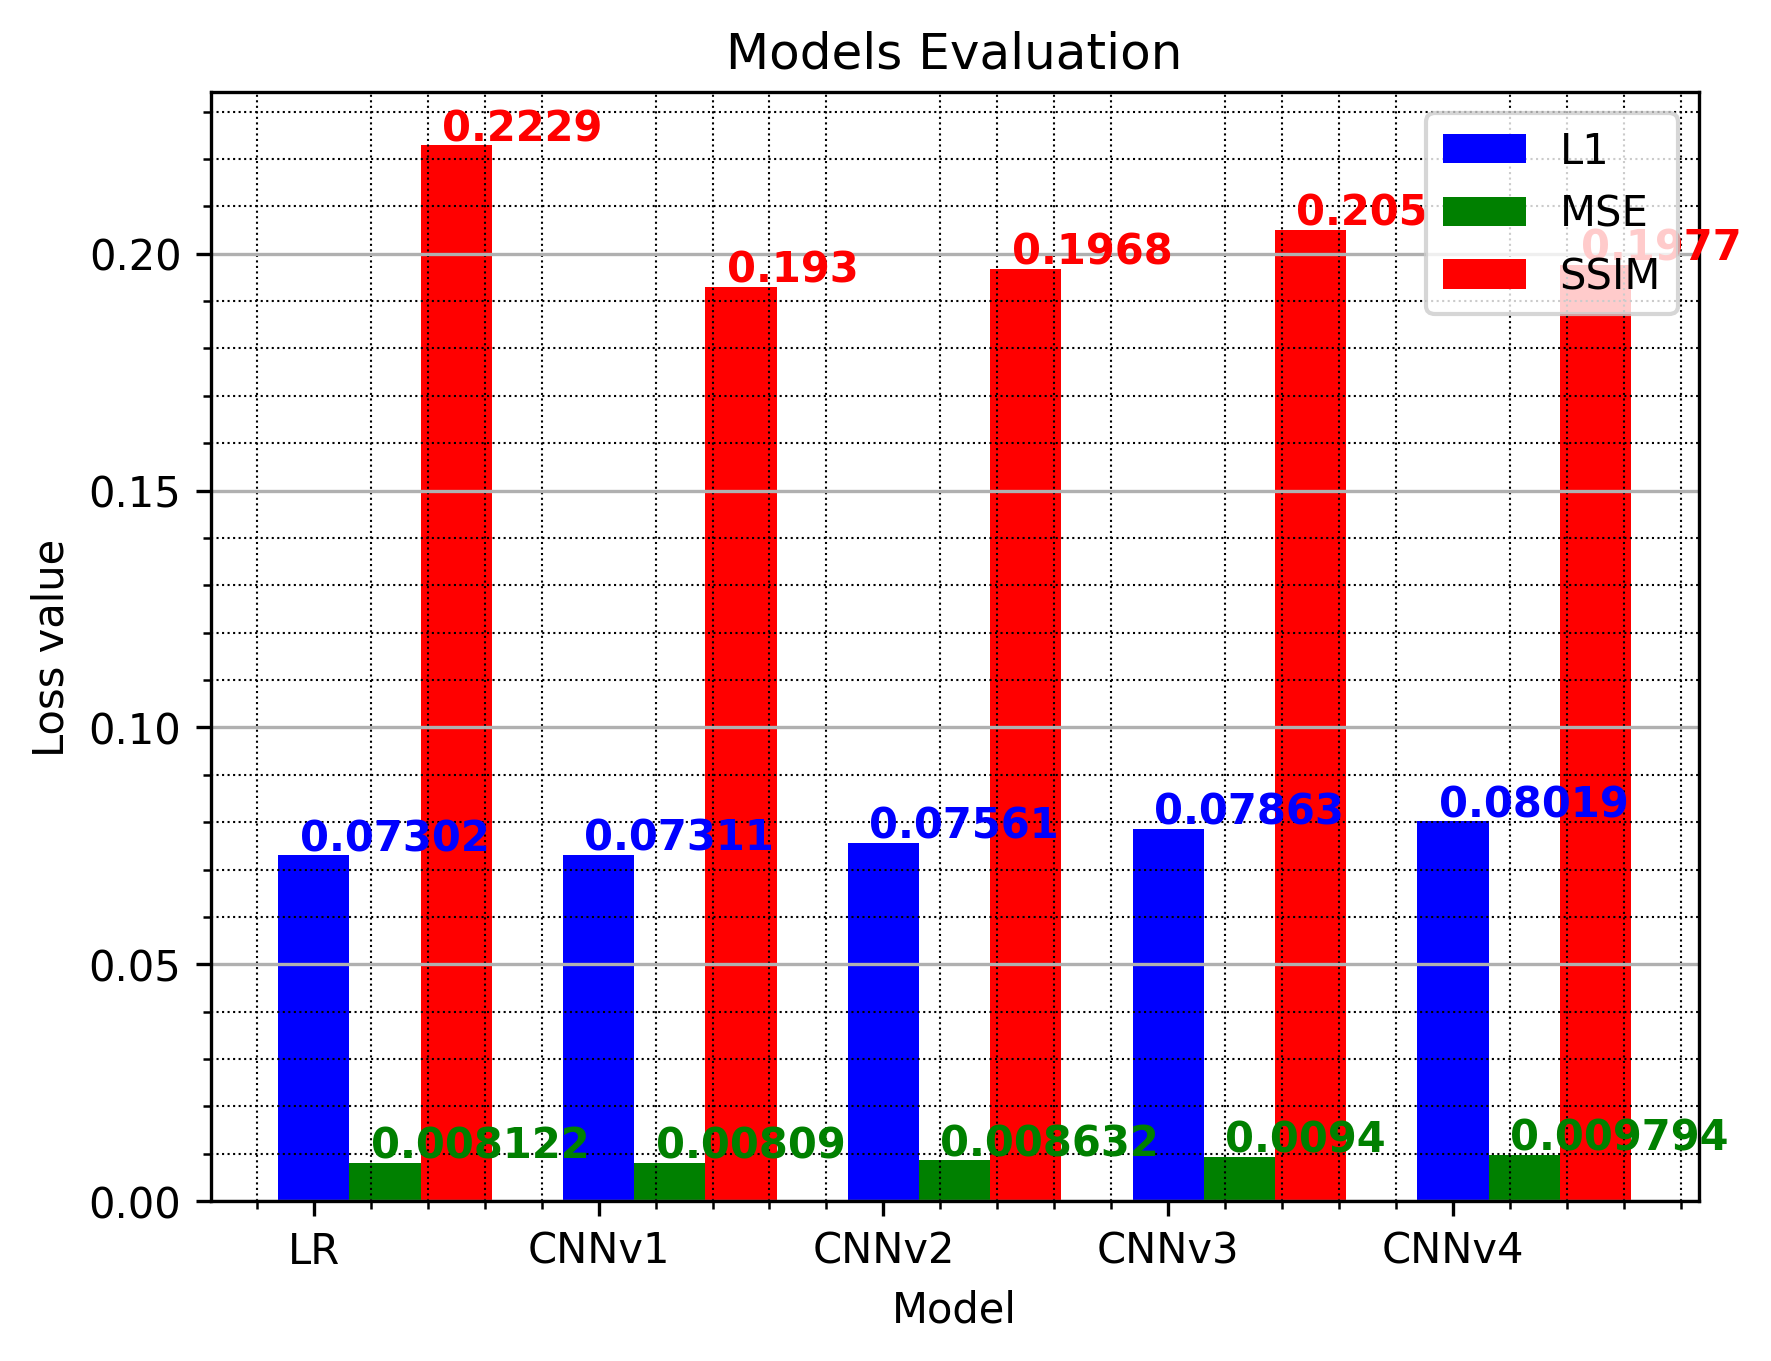
\includegraphics[width=140mm]{img/models_evaluation_ten_trials.png}
\caption{Comparison of multiple models on the same (ten-trials) dataset using different loss metrics.}
\label{img:experiments:ten-trials:comparison-outputs}
\end{figure}

On the image~\ref{img:experiments:ten-trials:comparison-outputs}, we see a comparison of the model outputs for two different cortical activity inputs on two testing samples. The first column contains the required stimulus image, and the rest of the columns correspond to each individual model. The second column to the linear regression model, the third one to CNNv1, and so on as described in the captions. We see that the LR and CNNv3 models try to reconstruct in a more detailed/localized way than the other models, although the reason of this behavior remains unclear.

All the models (except LR) were trained using MSSSIM loss (we present the reasons for using this loss in section~\ref{experiments:one-trial:finding-best-loss}). From the reconstructed images we can see, only a very limited number of low frequencies are being reconstructed. Interestingly, all the models, although independent, produce a similar reconstruction.


% **************************************************
\subsection{Linear Regression Dataset Size}
\label{experiments:ten-trials:linear-regression}
We tried to limit the number of data that were used to train the linear regression model~\ref{experiments:ten-trials:linear-regression}. We found that for this model, the loss function ($L_1$ in this case) value improved as the number of training data increased in the dataset until the maximum number of samples limit (3500 samples) was hit. We used linear regression for this task as the training is fully deterministic in comparison to CNN models, it is the fastest model to train on this dataset and the linear regression model performed best in terms of $L_1$, as described in~\ref{experiments:ten-trials}.

\begin{figure}[H]\centering
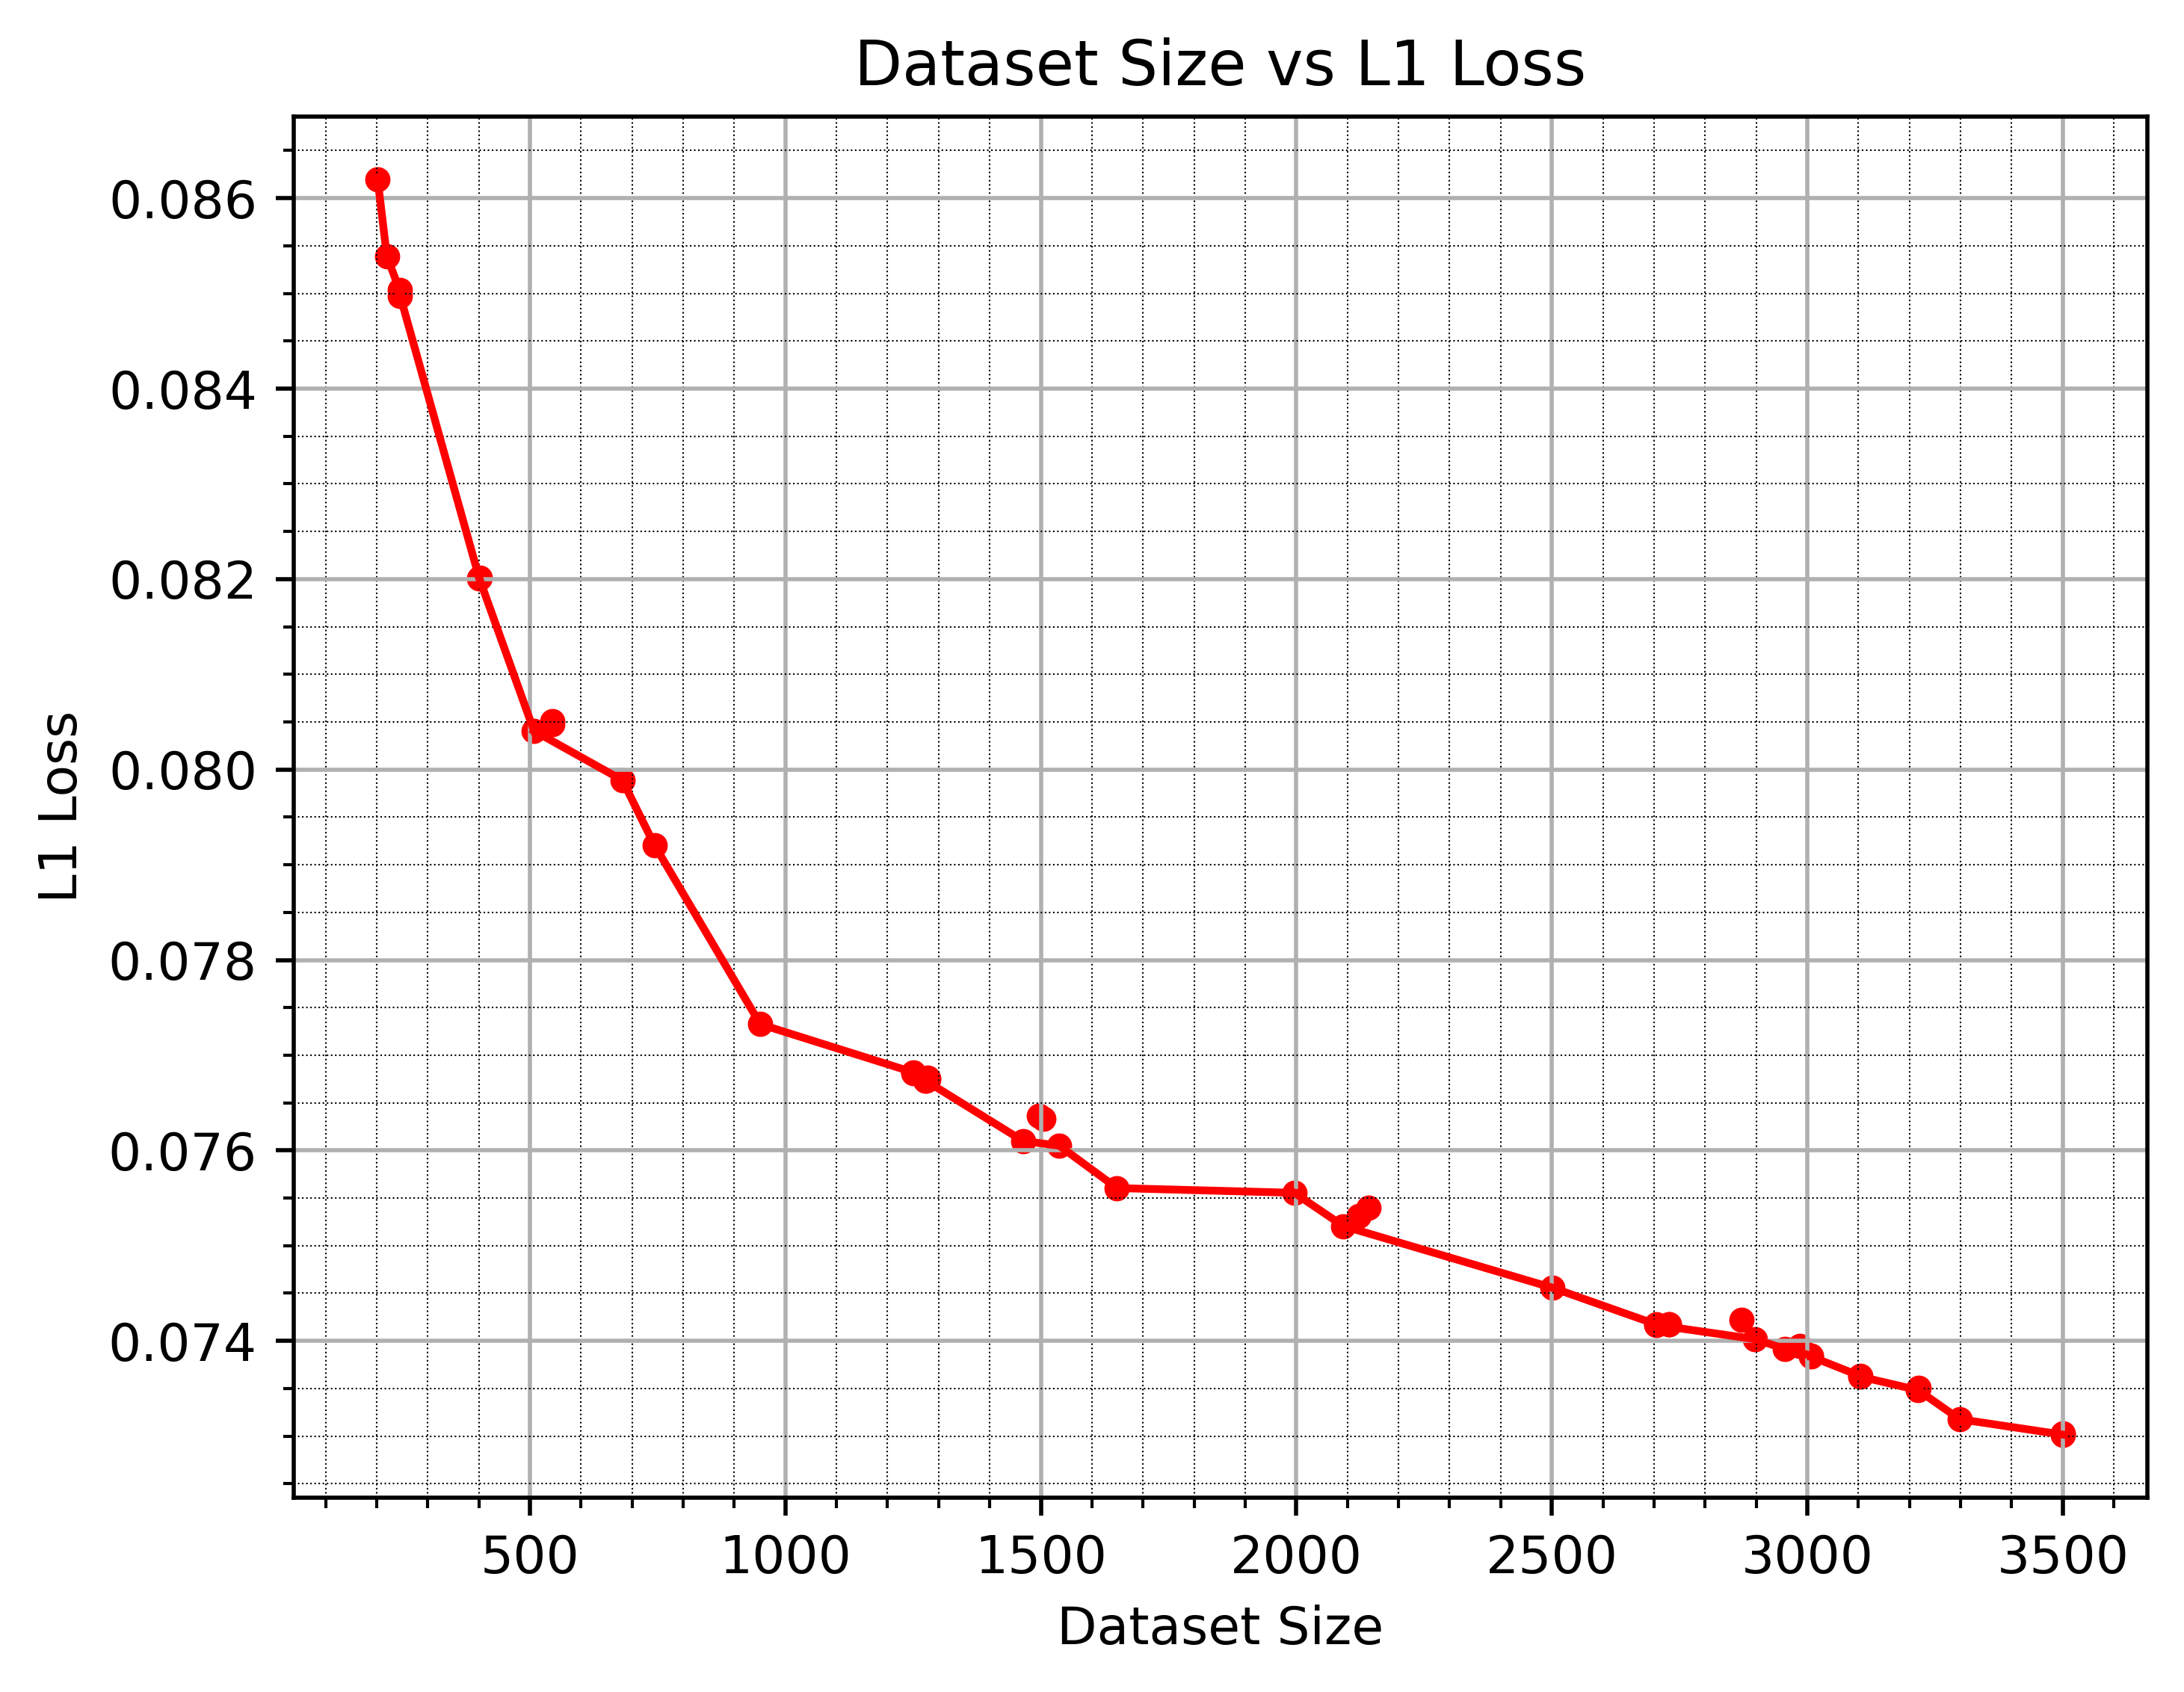
\includegraphics[width=140mm]{img/ten-trials/linear_regression_ten_trials.png}
\caption{Dependency of $L_1$ loss on the number of data in the training set for the linear regression model.}
\label{img:experiments:ten-trials:linear-regression}
\end{figure}

From this experiment, we conclude that the number of images is very important for the decoding of the stimuli. With a bigger dataset, it should be possible to perform better decoding.


% **************************************************
\subsection{Intristic Noise Limitation}
\label{experiments:ten-trials:intristic-noise-limitation}
To investigate if the intrinsic noise in neural responses represents a limitation for stimuli decoding, we used the best model for this dataset. Recall that we found that best model is the simple linear regression model (section~\ref{experiments:ten-trials}).

To find the answer to this question, use the following data:
\begin{description}
    \item[original] This dataset is unchanged, therefore contains each stimulus image ten-times with a different cortical response, meaning 3500 training samples (\ref{dataset:ten-trials}).
    \item[averaged] The same dataset, but the samples contain only unique stimuli images, each is crated by averaging the samples (responses) with the same stimulus image, therefore containing 350 samples for training. (The same is done for validation and testing samples.) The average is used here to remove the noise in the neural responses.
\end{description}

We then train two LR models:
\begin{enumerate}
    \item model, which is trained on all samples (\textbf{original} dataset)
    \item model, which is trained on averaged samples (\textbf{averaged} dataset)
\end{enumerate}

We already know, that the first model has $L_1$ loss of value $0.07304$ (\ref{experiments:ten-trials}). If we test the second model on the \textbf{averaged} dataset, we get $L_1$ value $0.07152$. From this, we conclude that the intristic noise in the neural responses represents a limitation for stimuli decoding, as we are able to get lower loss value by averaging the noisy samples across multiple trials. However, note that the improvement is not very significant.


% ==================================================
\section{One-trial Dataset}
\label{experiments:one-trial}
For the rest of the experiments, we will use the one-trial dataset~\ref{dataset:one-trial}, which is bigger than the ten-trials dataset and thus provides a better space for an improvement of the CNN models.


%% **************************************************
%\subsection{Linear Regression}
%\label{experiments:one-trial:linear-regression}
%\todo{description}


% **************************************************
\subsection{Finding Best Model}
\label{experiments:one-trial:finding-best-model}
To find the best-performing model, we trained all the model architectures described in~\ref{methods:models} on the training part of the one-trial dataset, we selected the best model state based on the validation part of the dataset and evaluated the results on the testing part of the dataset using the 4 main presented losses~\ref{methods:losses}.


\begin{figure}[H]\centering
  \begin{subfigure}[t]{0.45\textwidth}
    \centering
    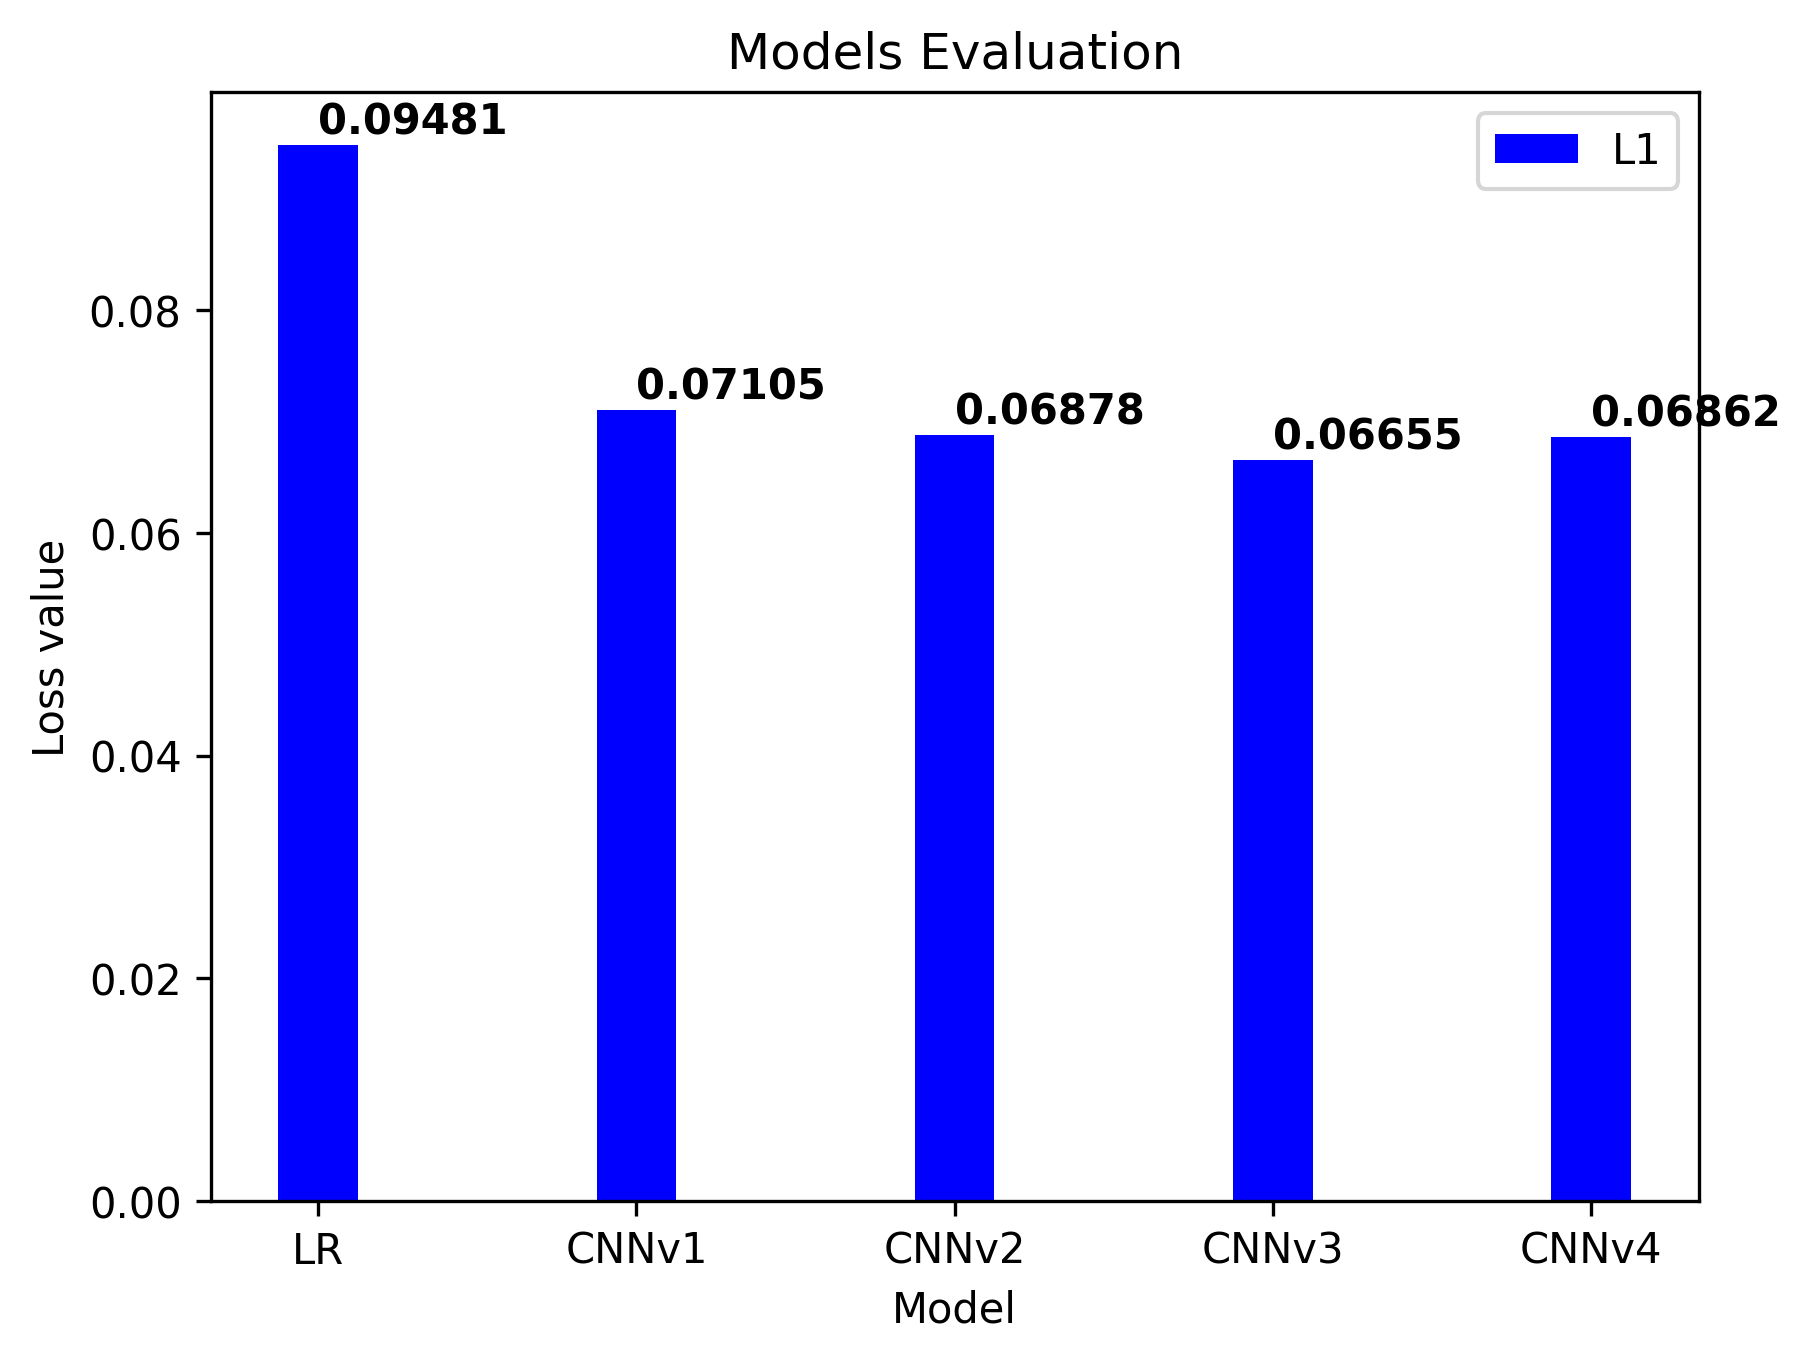
\includegraphics[width=\linewidth]{img/one-trial/models_evaluation_one_trial_l1.png}
    \caption{Models evaluation on $L_1$.}
  \end{subfigure}
  \begin{subfigure}[t]{0.45\textwidth}
    \centering
    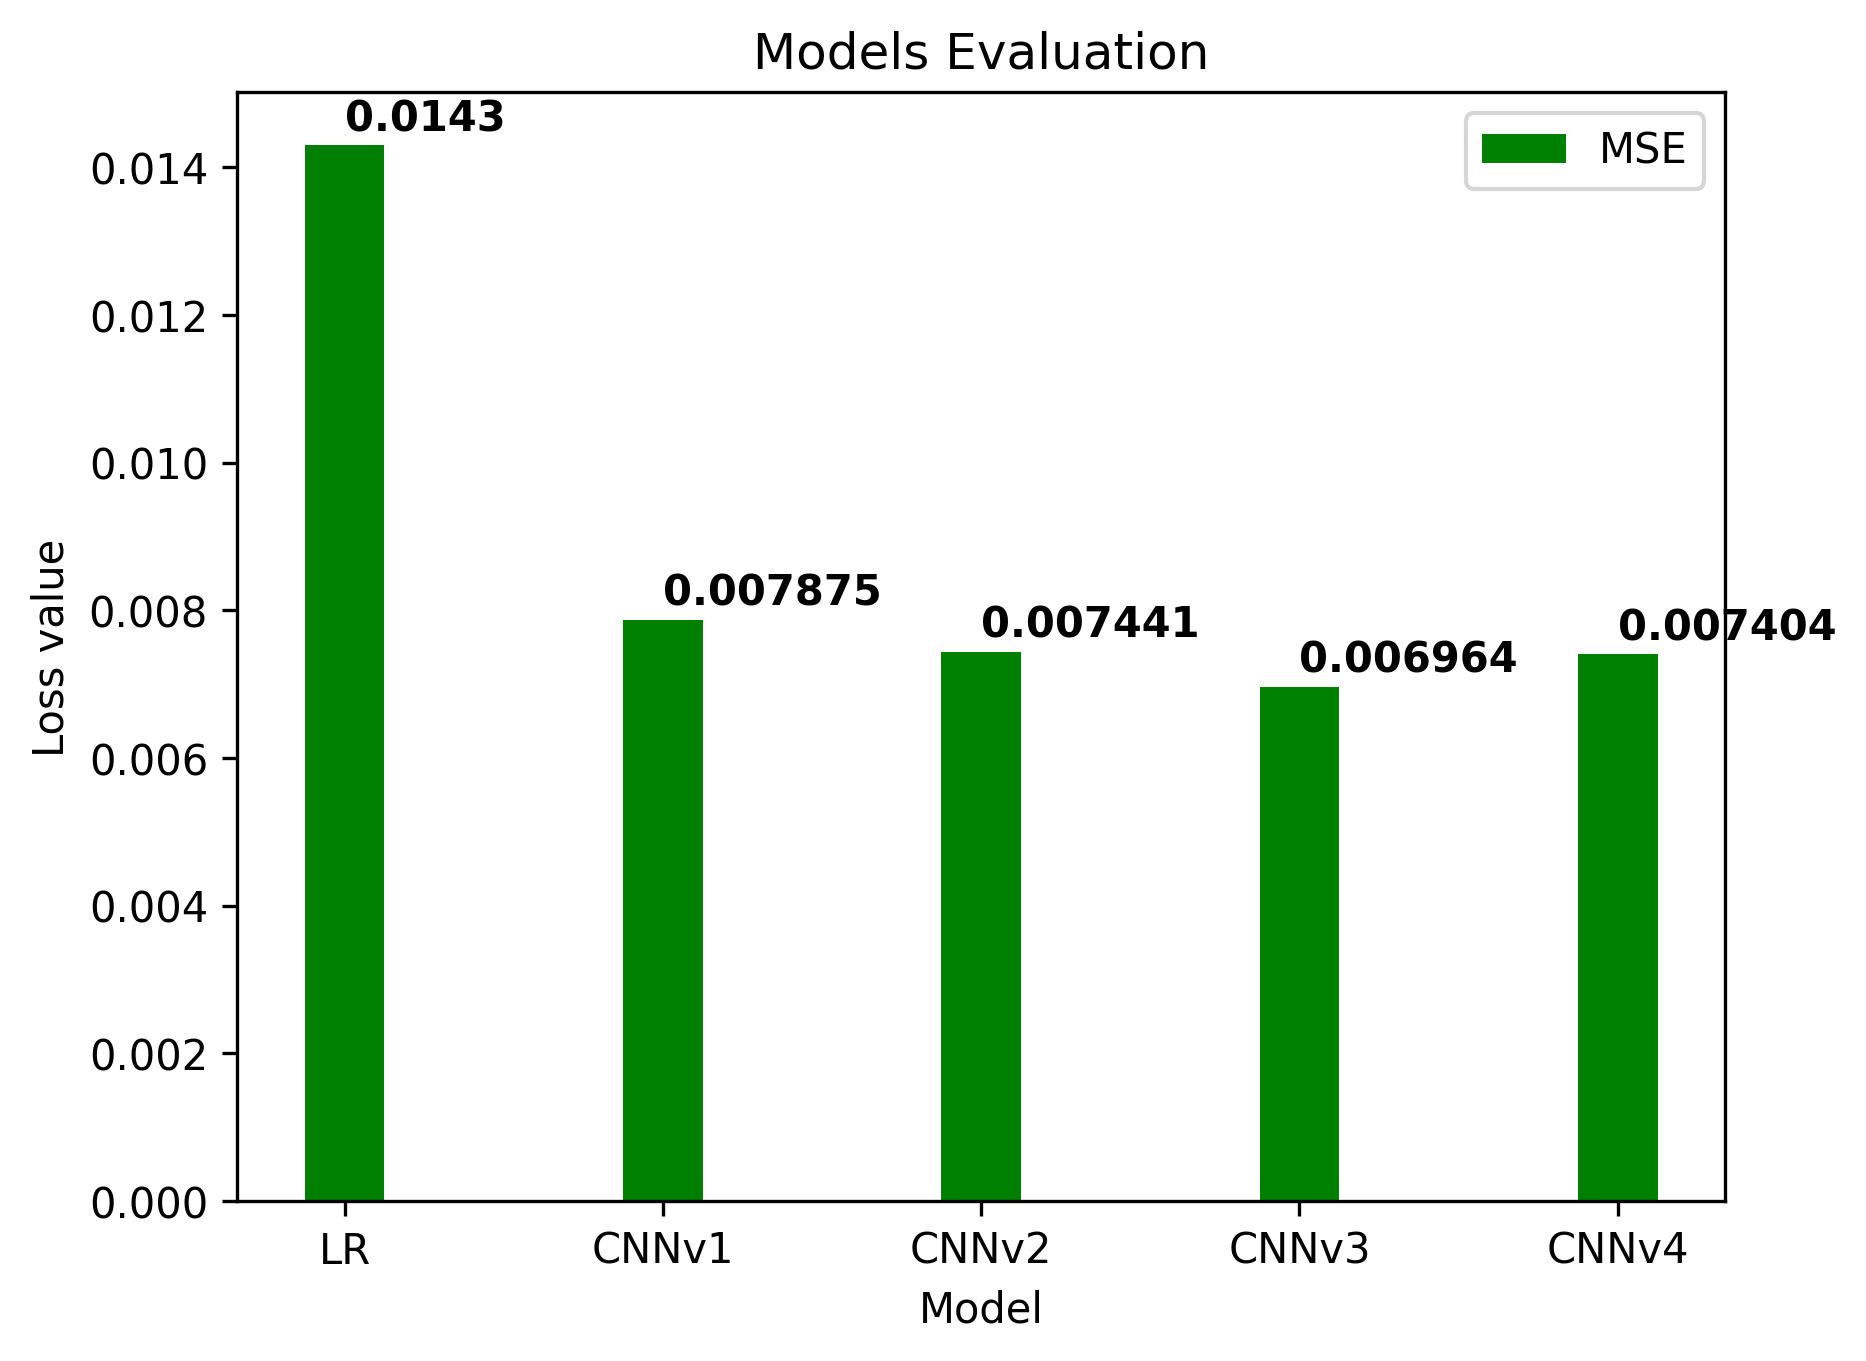
\includegraphics[width=\linewidth]{img/one-trial/models_evaluation_one_trial_mse.png}
    \caption{Models evaluation on MSE.}
  \end{subfigure}
  \\
  \begin{subfigure}[t]{0.45\textwidth}
    \centering
    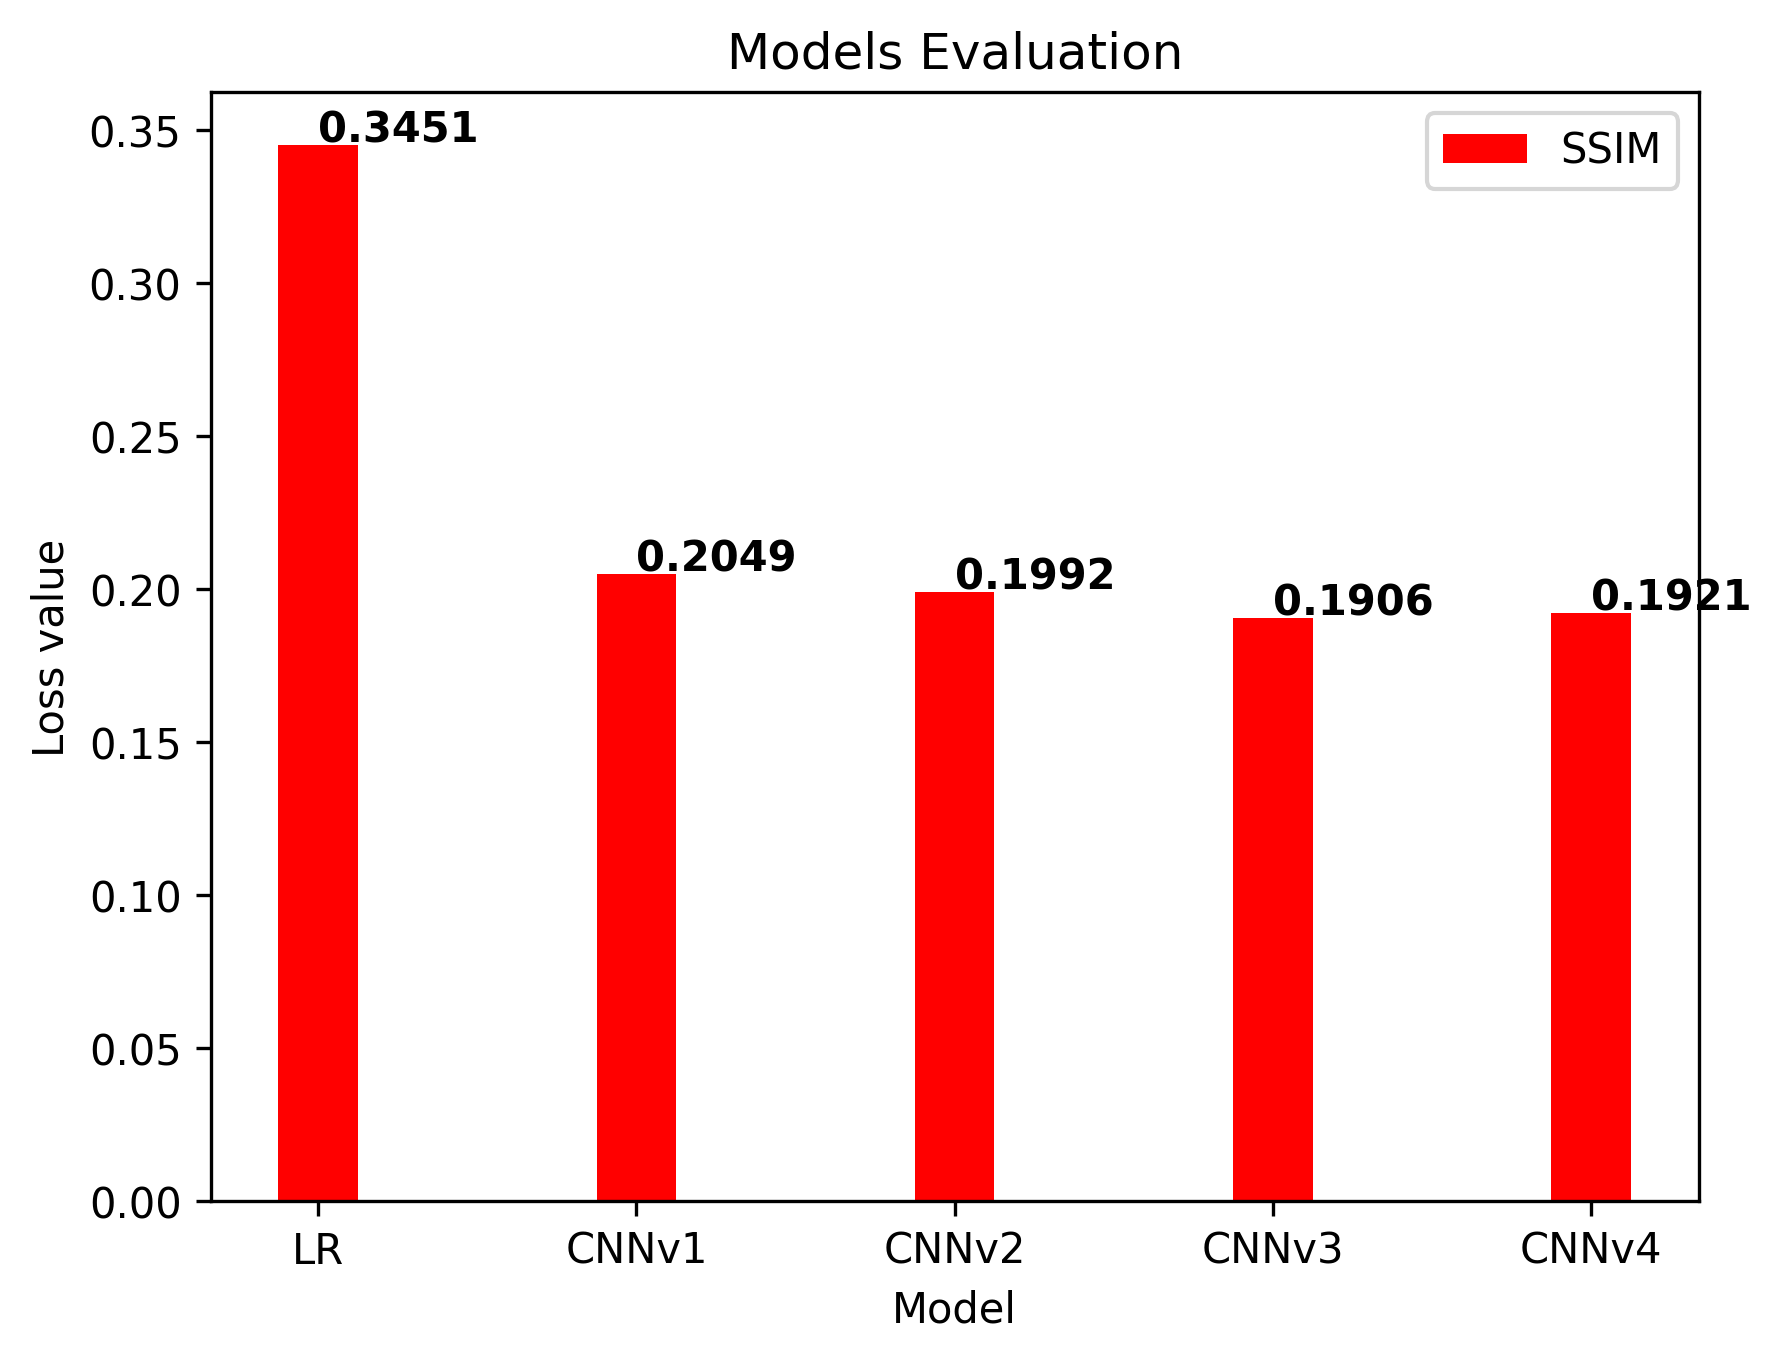
\includegraphics[width=\linewidth]{img/one-trial/models_evaluation_one_trial_ssim.png}
    \caption{Models evaluation on SSIM.}
  \end{subfigure}
  \begin{subfigure}[t]{0.45\textwidth}
    \centering
    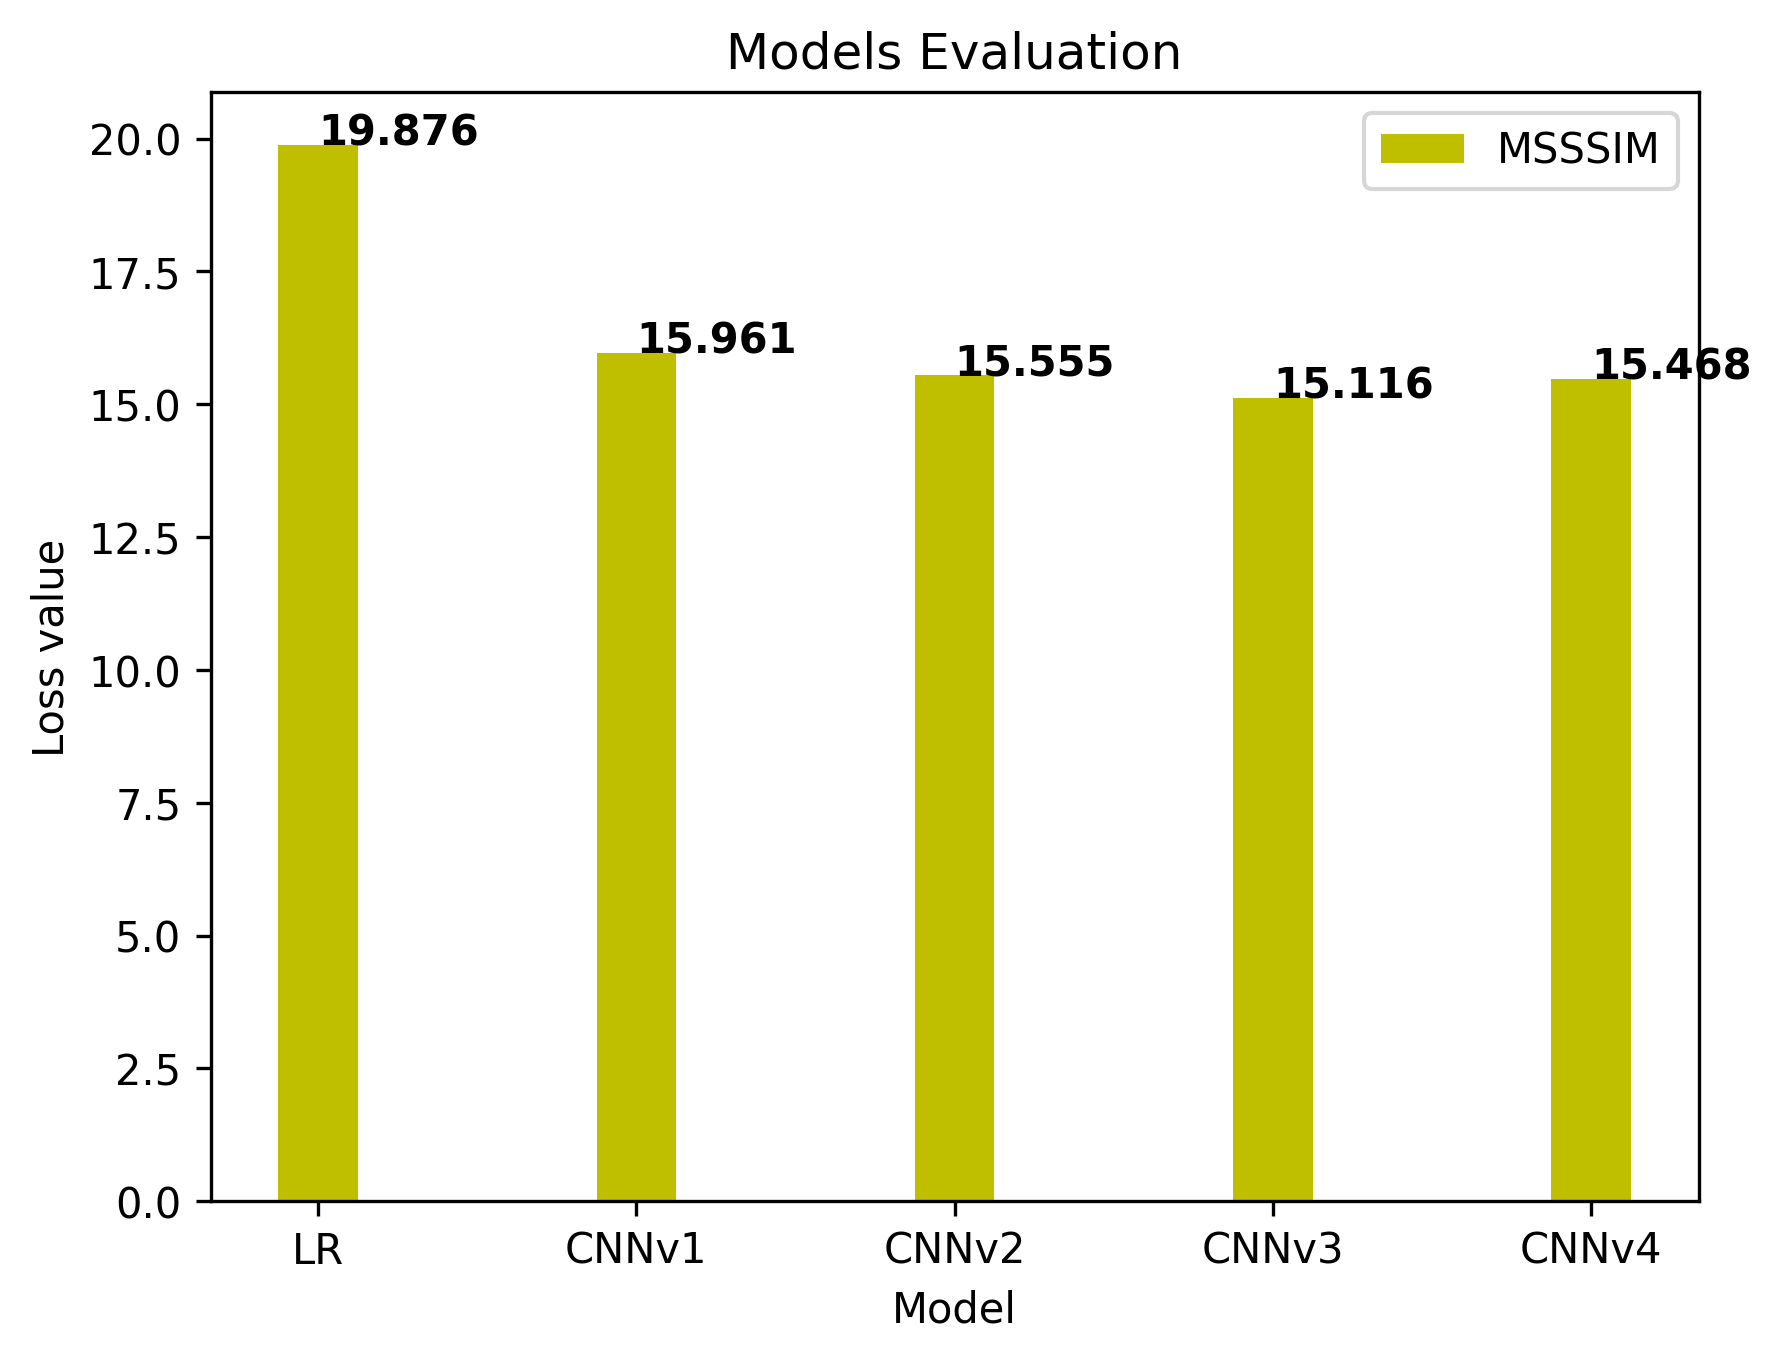
\includegraphics[width=\linewidth]{img/one-trial/models_evaluation_one_trial_msssim.png}
    \caption{Models evaluation on MSSSIM.}
  \end{subfigure}
\caption{Comparison of multiple models on the same (one-trial) dataset using different loss metrics.}
\label{img:experiments:one-trial:comparison}
\end{figure}

On the picture~\ref{img:experiments:one-trial:comparison}, we can see the results separately for $L_1$, MSE, SSIM, and MSSSIM losses. It is clear, that the linear regression model is now the worst, as all the losses are highest for it. On the other hand, we can see that the CNN model's performance is quite similar. The best one of them is model CNNv3, which is slightly better than CNNv4, then we have CNNv2 and CNNv1 is the worst of the CNN models by all four metrics.

\begin{figure}[H]\centering

  \begin{subfigure}[t]{0.15\textwidth}
    \centering
    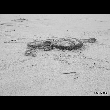
\includegraphics[width=\linewidth]{img/one-trial/stimulus_1.png}
    % \caption{Stim. 1}
  \end{subfigure}
  \begin{subfigure}[t]{0.15\textwidth}
    \centering
    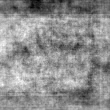
\includegraphics[width=\linewidth]{img/one-trial/prediction_1_lr.png}
    % \caption{LR}
  \end{subfigure}
  \begin{subfigure}[t]{0.15\textwidth}
    \centering
    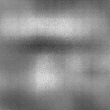
\includegraphics[width=\linewidth]{img/one-trial/prediction_1_cnnv1.png}
    % \caption{CNNv1}
  \end{subfigure}
  \begin{subfigure}[t]{0.15\textwidth}
    \centering
    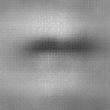
\includegraphics[width=\linewidth]{img/one-trial/prediction_1_cnnv2.png}
    % \caption{CNNv2}
  \end{subfigure}
  \begin{subfigure}[t]{0.15\textwidth}
    \centering
    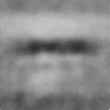
\includegraphics[width=\linewidth]{img/one-trial/prediction_1_cnnv3.png}
    % \caption{CNNv3}
  \end{subfigure}
  \begin{subfigure}[t]{0.15\textwidth}
    \centering
    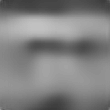
\includegraphics[width=\linewidth]{img/one-trial/prediction_1_cnnv4.png}
    % \caption{CNNv4}
  \end{subfigure}
  \\
    \vspace{0.1cm}
  
  \begin{subfigure}[t]{0.15\textwidth}
    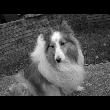
\includegraphics[width=\linewidth]{img/one-trial/stimulus_2.png}
    % \caption{Stim. 2}
  \end{subfigure}
  \begin{subfigure}[t]{0.15\textwidth}
    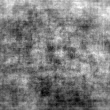
\includegraphics[width=\linewidth]{img/one-trial/prediction_2_lr.png}
    % \caption{LR}
  \end{subfigure}
  \begin{subfigure}[t]{0.15\textwidth}
    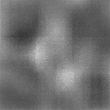
\includegraphics[width=\linewidth]{img/one-trial/prediction_2_cnnv1.png}
    % \caption{CNNv1}
  \end{subfigure}
  \begin{subfigure}[t]{0.15\textwidth}
    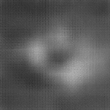
\includegraphics[width=\linewidth]{img/one-trial/prediction_2_cnnv2.png}
    % \caption{CNNv2}
  \end{subfigure}
  \begin{subfigure}[t]{0.15\textwidth}
    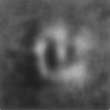
\includegraphics[width=\linewidth]{img/one-trial/prediction_2_cnnv3.png}
    % \caption{CNNv3}
  \end{subfigure}
  \begin{subfigure}[t]{0.15\textwidth}
    
\includegraphics[width=\linewidth]{img/one-trial/prediction_2_cnnv4.png}
    % \caption{CNNv4}
  \end{subfigure}
  \\
    \vspace{0.1cm}
  
  \begin{subfigure}[t]{0.15\textwidth}
    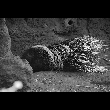
\includegraphics[width=\linewidth]{img/one-trial/stimulus_3.png}
    % \caption{Stim. 3}
  \end{subfigure}
  \begin{subfigure}[t]{0.15\textwidth}
    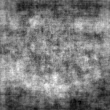
\includegraphics[width=\linewidth]{img/one-trial/prediction_3_lr.png}
    % \caption{LR}
  \end{subfigure}
  \begin{subfigure}[t]{0.15\textwidth}
    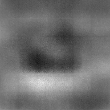
\includegraphics[width=\linewidth]{img/one-trial/prediction_3_cnnv1.png}
    % \caption{CNNv1}
  \end{subfigure}
  \begin{subfigure}[t]{0.15\textwidth}
    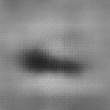
\includegraphics[width=\linewidth]{img/one-trial/prediction_3_cnnv2.png}
    % \caption{CNNv2}
  \end{subfigure}
  \begin{subfigure}[t]{0.15\textwidth}
    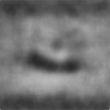
\includegraphics[width=\linewidth]{img/one-trial/prediction_3_cnnv3.png}
    % \caption{CNNv3}
  \end{subfigure}
  \begin{subfigure}[t]{0.15\textwidth}
    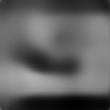
\includegraphics[width=\linewidth]{img/one-trial/prediction_3_cnnv4.png}
    % \caption{CNNv4}
  \end{subfigure}
  \\
    \vspace{0.1cm}
  
  \begin{subfigure}[t]{0.15\textwidth}
    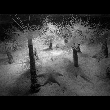
\includegraphics[width=\linewidth]{img/one-trial/stimulus_4.png}
    \caption{Stimuli}
  \end{subfigure}
  \begin{subfigure}[t]{0.15\textwidth}
    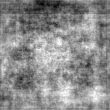
\includegraphics[width=\linewidth]{img/one-trial/prediction_4_lr.png}
    \caption{LR}
  \end{subfigure}
  \begin{subfigure}[t]{0.15\textwidth}
    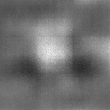
\includegraphics[width=\linewidth]{img/one-trial/prediction_4_cnnv1.png}
    \caption{CNNv1}
  \end{subfigure}
  \begin{subfigure}[t]{0.15\textwidth}
    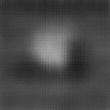
\includegraphics[width=\linewidth]{img/one-trial/prediction_4_cnnv2.png}
    \caption{CNNv2}
  \end{subfigure}
  \begin{subfigure}[t]{0.15\textwidth}
    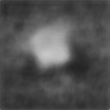
\includegraphics[width=\linewidth]{img/one-trial/prediction_4_cnnv3.png}
    \caption{CNNv3}
  \end{subfigure}
  \begin{subfigure}[t]{0.15\textwidth}
    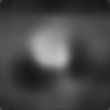
\includegraphics[width=\linewidth]{img/one-trial/prediction_4_cnnv4.png}
    \caption{CNNv4}
  \end{subfigure}
  
\caption{Visual comparison of multiple models on the same cortical activity samples. Each row corresponds to one sample. The first column contains the stimuli targets, each column shows images generated by a different model.}
\label{img:experiments:one-trial:comparison-outputs}
\end{figure}

To better understand the difference in the predictions, we also provide sample outputs for four different cortical activity inputs from the testing part of the dataset~\ref{img:experiments:one-trial:comparison-outputs}. The outputs of the linear regression model look very noisy. The CNNv3 gives results that are convincing both in the loss metrics and also when we compare them visually.

From now on, we use only the best model (CNNv3) to perform the rest of the experiments, which use only one model.


% **************************************************
\subsection{Intermediate Image}
\label{experiments:one-trial:intermediate-image}
Two of our implemented architectures use intermediate images inside the network, namely CNNv3~\ref{methods:models:CNNv3} and CNNv4~\ref{methods:models:CNNv4}. The CNNv3 uses a stack of transposed convolutional layers on top of the intermediate image to produce the output image. CNNv4 instead uses an encoder-decoder type of network to denoise the intermediate image~\citep{zhang2020reconstruction}. We show the intermediate images together with stimuli and output images in the figure~\ref{img:experiments:one-trial:intermediate-image}.


\begin{figure}[H]\centering
  \setcounter{subfigure}{0}
  \begin{subfigure}[t]{0.13\textwidth}
    \centering
    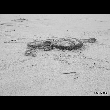
\includegraphics[width=\linewidth]{img/one-trial/stimulus_1.png}
    % \caption{Stim. 1}
  \end{subfigure}
  \begin{subfigure}[t]{0.13\textwidth}
    \centering
    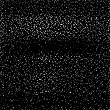
\includegraphics[width=\linewidth]{img/one-trial/intermediate-cnnv3/intermediate_0.png}
    % \caption{CNNv3}
  \end{subfigure}
  \begin{subfigure}[t]{0.13\textwidth}
    \centering
    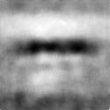
\includegraphics[width=\linewidth]{img/one-trial/intermediate-cnnv3/prediction_0.png}
    % \caption{CNNv3}
  \end{subfigure}
  \begin{subfigure}[t]{0.13\textwidth}
    \centering
    \includegraphics[width=\linewidth]{img/one-trial/intermediate-cnnv4/intermediate_0.png}
    % \caption{CNNv4}
  \end{subfigure}
  \begin{subfigure}[t]{0.13\textwidth}
    \centering
    \includegraphics[width=\linewidth]{img/one-trial/intermediate-cnnv4/prediction_0.png}
    % \caption{CNNv4}
  \end{subfigure}
  \\
    \vspace{0.1cm}
  
  \setcounter{subfigure}{0}
  \begin{subfigure}[t]{0.13\textwidth}
    \centering
    \includegraphics[width=\linewidth]{img/one-trial/stimulus_2.png}
    % \caption{Stim. 1}
  \end{subfigure}
  \begin{subfigure}[t]{0.13\textwidth}
    \centering
    \includegraphics[width=\linewidth]{img/one-trial/intermediate-cnnv3/intermediate_1.png}
    % \caption{CNNv3}
  \end{subfigure}
  \begin{subfigure}[t]{0.13\textwidth}
    \centering
    \includegraphics[width=\linewidth]{img/one-trial/intermediate-cnnv3/prediction_1.png}
    % \caption{CNNv3}
  \end{subfigure}
  \begin{subfigure}[t]{0.13\textwidth}
    \centering
    \includegraphics[width=\linewidth]{img/one-trial/intermediate-cnnv4/intermediate_1.png}
    % \caption{CNNv4}
  \end{subfigure}
  \begin{subfigure}[t]{0.13\textwidth}
    \centering
    \includegraphics[width=\linewidth]{img/one-trial/intermediate-cnnv4/prediction_1.png}
    % \caption{CNNv4}
  \end{subfigure}
  \\
    \vspace{0.1cm}
  
  \setcounter{subfigure}{0}
  \begin{subfigure}[t]{0.13\textwidth}
    \centering
    \includegraphics[width=\linewidth]{img/one-trial/stimulus_3.png}
    % \caption{Stim. 1}
  \end{subfigure}
  \begin{subfigure}[t]{0.13\textwidth}
    \centering
    \includegraphics[width=\linewidth]{img/one-trial/intermediate-cnnv3/intermediate_2.png}
    % \caption{CNNv3}
  \end{subfigure}
  \begin{subfigure}[t]{0.13\textwidth}
    \centering
    \includegraphics[width=\linewidth]{img/one-trial/intermediate-cnnv3/prediction_2.png}
    % \caption{CNNv3}
  \end{subfigure}
  \begin{subfigure}[t]{0.13\textwidth}
    \centering
    \includegraphics[width=\linewidth]{img/one-trial/intermediate-cnnv4/intermediate_2.png}
    % \caption{CNNv4}
  \end{subfigure}
  \begin{subfigure}[t]{0.13\textwidth}
    \centering
    \includegraphics[width=\linewidth]{img/one-trial/intermediate-cnnv4/prediction_2.png}
    % \caption{CNNv4}
  \end{subfigure}
  \\
    \vspace{0.1cm}
  
  \setcounter{subfigure}{0}
  \begin{subfigure}[t]{0.13\textwidth}
    \centering
    \includegraphics[width=\linewidth]{img/one-trial/stimulus_4.png}
    \caption{Stimuli}
  \end{subfigure}
  \begin{subfigure}[t]{0.13\textwidth}
    \centering
    \includegraphics[width=\linewidth]{img/one-trial/intermediate-cnnv3/intermediate_3.png}
    \caption{CNNv3}
  \end{subfigure}
  \begin{subfigure}[t]{0.13\textwidth}
    \centering
    \includegraphics[width=\linewidth]{img/one-trial/intermediate-cnnv3/prediction_3.png}
    \caption{CNNv3}
  \end{subfigure}
  \begin{subfigure}[t]{0.13\textwidth}
    \centering
    \includegraphics[width=\linewidth]{img/one-trial/intermediate-cnnv4/intermediate_3.png}
    \caption{CNNv4}
  \end{subfigure}
  \begin{subfigure}[t]{0.13\textwidth}
    \centering
    \includegraphics[width=\linewidth]{img/one-trial/intermediate-cnnv4/prediction_3.png}
    \caption{CNNv4}
  \end{subfigure}
  
\caption{Table of images for visual comparison of stimuli images (first column), intermediate images (columns b and d), and the actual output of the models (columns c and e). Each row represents a different sample, columns b and c are generated by model CNNv3, and columns d and e by model CNNv4.}
\label{img:experiments:one-trial:intermediate-image}
\end{figure}

Based on the intermediate images, we conclude that the model CNNv3 is producing an image that is much closer to the one which is then generated as an output, although it contains much more noise than the output image. The model CNNv4 is generating an intermediate image, which looks very noisy, there is no visual similarity with the output and the idea to use the encoder-decoder architecture to enhance the intermediate image is therefore questionable.


% **************************************************
\subsection{Finding Best Loss Function}
\label{experiments:one-trial:finding-best-loss}
We used the CNNv3 model and trained it using all the loss functions defined in~\ref{methods:losses}. The results are on plots~\ref{img:experiments:one-trial:finding-best-loss-bars}.

\begin{figure}[H]\centering
  \begin{subfigure}[t]{0.45\textwidth}
    \centering
    \includegraphics[width=\linewidth]{img/one-trial/model_loss_one_trial_l1.png}
    \caption{Models evaluation on $L_1$.}
  \end{subfigure}
  \begin{subfigure}[t]{0.45\textwidth}
    \centering
    \includegraphics[width=\linewidth]{img/one-trial/model_loss_one_trial_mse.png}
    \caption{Models evaluation on MSE.}
  \end{subfigure}
  \\
  \begin{subfigure}[t]{0.45\textwidth}
    \centering
    \includegraphics[width=\linewidth]{img/one-trial/model_loss_one_trial_ssim.png}
    \caption{Models evaluation on SSIM.}
  \end{subfigure}
  \begin{subfigure}[t]{0.45\textwidth}
    \centering
    \includegraphics[width=\linewidth]{img/one-trial/model_loss_one_trial_msssim.png}
    \caption{Models evaluation on MSSSIM.}
  \end{subfigure}
\caption{Comparison showing how final testing/validation loss depends on different training losses.}
\label{img:experiments:one-trial:finding-best-loss-bars}
\end{figure}

Interestingly we found that no matter which of the four main loss metrics is used as the target one, we get the best results when we train using the MSSSIM loss. We also show how the results differ when we use different training losses visually on picture~\ref{img:experiments:one-trial:finding-best-loss-outputs}.

\begin{figure}[H]\centering
  \setcounter{subfigure}{0}
  \begin{subfigure}[t]{0.13\textwidth}
    \centering
    \includegraphics[width=\linewidth]{img/one-trial/stimulus_1.png}
    % \caption{Stim. 1}
  \end{subfigure}
  \begin{subfigure}[t]{0.13\textwidth}
    \centering
    \includegraphics[width=\linewidth]{img/one-trial/prediction_1_l1.png}
    % \caption{L1}
  \end{subfigure}
  \begin{subfigure}[t]{0.13\textwidth}
    \centering
    \includegraphics[width=\linewidth]{img/one-trial/prediction_1_mse.png}
    % \caption{MSE}
  \end{subfigure}
  \begin{subfigure}[t]{0.13\textwidth}
    \centering
    \includegraphics[width=\linewidth]{img/one-trial/prediction_1_ssim.png}
    % \caption{SSIM}
  \end{subfigure}
  \begin{subfigure}[t]{0.13\textwidth}
    \centering
    \includegraphics[width=\linewidth]{img/one-trial/prediction_1_msssim.png}
    % \caption{MSSSIM}
  \end{subfigure}
  \begin{subfigure}[t]{0.13\textwidth}
    \centering
    \includegraphics[width=\linewidth]{img/one-trial/prediction_1_mix.png}
    % \caption{MIX}
  \end{subfigure}
  \begin{subfigure}[t]{0.13\textwidth}
    \centering
    \includegraphics[width=\linewidth]{img/one-trial/prediction_1_adversarial.png}
    % \caption{Adversarial}
  \end{subfigure}
  \\
    \vspace{0.1cm}
  
  \setcounter{subfigure}{0}
  \begin{subfigure}[t]{0.13\textwidth}
    \centering
    \includegraphics[width=\linewidth]{img/one-trial/stimulus_2.png}
    % \caption{Stim. 1}
  \end{subfigure}
  \begin{subfigure}[t]{0.13\textwidth}
    \centering
    \includegraphics[width=\linewidth]{img/one-trial/prediction_2_l1.png}
    % \caption{L1}
  \end{subfigure}
  \begin{subfigure}[t]{0.13\textwidth}
    \centering
    \includegraphics[width=\linewidth]{img/one-trial/prediction_2_mse.png}
    % \caption{MSE}
  \end{subfigure}
  \begin{subfigure}[t]{0.13\textwidth}
    \centering
    \includegraphics[width=\linewidth]{img/one-trial/prediction_2_ssim.png}
    % \caption{SSIM}
  \end{subfigure}
  \begin{subfigure}[t]{0.13\textwidth}
    \centering
    \includegraphics[width=\linewidth]{img/one-trial/prediction_2_msssim.png}
    % \caption{MSSSIM}
  \end{subfigure}
  \begin{subfigure}[t]{0.13\textwidth}
    \centering
    \includegraphics[width=\linewidth]{img/one-trial/prediction_2_mix.png}
    % \caption{MIX}
  \end{subfigure}
  \begin{subfigure}[t]{0.13\textwidth}
    \centering
    \includegraphics[width=\linewidth]{img/one-trial/prediction_2_adversarial.png}
    % \caption{Adversarial}
  \end{subfigure}
  \\
    \vspace{0.1cm}
  
  \setcounter{subfigure}{0}
  \begin{subfigure}[t]{0.13\textwidth}
    \centering
    \includegraphics[width=\linewidth]{img/one-trial/stimulus_3.png}
    % \caption{Stim. 1}
  \end{subfigure}
  \begin{subfigure}[t]{0.13\textwidth}
    \centering
    \includegraphics[width=\linewidth]{img/one-trial/prediction_3_l1.png}
    % \caption{L1}
  \end{subfigure}
  \begin{subfigure}[t]{0.13\textwidth}
    \centering
    \includegraphics[width=\linewidth]{img/one-trial/prediction_3_mse.png}
    % \caption{MSE}
  \end{subfigure}
  \begin{subfigure}[t]{0.13\textwidth}
    \centering
    \includegraphics[width=\linewidth]{img/one-trial/prediction_3_ssim.png}
    % \caption{SSIM}
  \end{subfigure}
  \begin{subfigure}[t]{0.13\textwidth}
    \centering
    \includegraphics[width=\linewidth]{img/one-trial/prediction_3_msssim.png}
    % \caption{MSSSIM}
  \end{subfigure}
  \begin{subfigure}[t]{0.13\textwidth}
    \centering
    \includegraphics[width=\linewidth]{img/one-trial/prediction_3_mix.png}
    % \caption{MIX}
  \end{subfigure}
  \begin{subfigure}[t]{0.13\textwidth}
    \centering
    \includegraphics[width=\linewidth]{img/one-trial/prediction_3_adversarial.png}
    % \caption{Adversarial}
  \end{subfigure}
  \\
    \vspace{0.1cm}
  
  \setcounter{subfigure}{0}
  \begin{subfigure}[t]{0.13\textwidth}
    \centering
    \includegraphics[width=\linewidth]{img/one-trial/stimulus_4.png}
    \caption{Stimuli}
  \end{subfigure}
  \begin{subfigure}[t]{0.13\textwidth}
    \centering
    \includegraphics[width=\linewidth]{img/one-trial/prediction_4_l1.png}
    \caption{L1}
  \end{subfigure}
  \begin{subfigure}[t]{0.13\textwidth}
    \centering
    \includegraphics[width=\linewidth]{img/one-trial/prediction_4_mse.png}
    \caption{MSE}
  \end{subfigure}
  \begin{subfigure}[t]{0.13\textwidth}
    \centering
    \includegraphics[width=\linewidth]{img/one-trial/prediction_4_ssim.png}
    \caption{SSIM}
  \end{subfigure}
  \begin{subfigure}[t]{0.13\textwidth}
    \centering
    \includegraphics[width=\linewidth]{img/one-trial/prediction_4_msssim.png}
    \caption{MSSSIM}
  \end{subfigure}
  \begin{subfigure}[t]{0.13\textwidth}
    \centering
    \includegraphics[width=\linewidth]{img/one-trial/prediction_4_mix.png}
    \caption{MIX}
  \end{subfigure}
  \begin{subfigure}[t]{0.13\textwidth}
    \centering
    \includegraphics[width=\linewidth]{img/one-trial/prediction_4_adversarial.png}
    \caption{Discriminator}
  \end{subfigure}
  
\caption{Visual comparison of multiple models, each trained with a different loss function. Each row corresponds to one sample. The first column contains the stimuli targets, other columns show images generated by different models.}
\label{img:experiments:one-trial:finding-best-loss-outputs}
\end{figure}

When compared visually, it corresponds also to the low value of loss metrics, that the model trained with MSSSIM loss is one of the best ones. The results of the discriminator loss also look like they can depict higher frequencies and contrast better, but this model does not look so well when measured by the loss metrics. We can therefore conclude, that the subjective human visual comparison can sometimes differ from the mathematical-based loss metrics.

% **************************************************
\subsection{Evaluating Dataset Size}
\label{experiments:one-trial:number-of-samples}
To inspect how important is to have enough samples when training the models, we did a sweep on the dataset size. For the given number of samples $n \in \mathbb{N}$, we selected only the first part of the training samples so that only the first $n$ samples were used. We trained only on those, selected the best model state based on the validation part, and evaluated on the same testing part. In other words, only the training set size was variable in each run.

The results are on image~\ref{img:experiments:one-trial:number-of-samples}. We observed that with more samples, the model was able to perform better in terms of the $L_1$ loss. We also observed some noise in the measurements (the values are not always decreasing monotonically) which was expected, as the training of the CNN models is not deterministic.

\begin{figure}[H]\centering
\includegraphics[width=140mm]{img/one-trial/dataset_size_one_trial.png}
\caption{Dependency of model $L_1$ loss on the size of the dataset in several training samples.}
\label{img:experiments:one-trial:number-of-samples}
\end{figure}


% **************************************************
\subsection{Exploring Number of Input Neurons}
\label{experiments:one-trial:number-of-inputs}
To show the importance of the cortical activity neurons, we did another sweep, where the variable was the number of neurons from the cortical activity, which the model was able to use. For each number of neurons, the neurons were selected randomly, the model was trained on the whole training part, the best model was selected using the validation set, and the results on the testing part were used to plot the values in this graph.

The results are on image~\ref{img:experiments:one-trial:number-of-inputs}. The maximum number of neurons is $60000$, which produces the best $L_1$ value. We can again see a dependency, which shows us that using more neurons helps the model to find a better solution.

\begin{figure}[H]\centering
\includegraphics[width=140mm]{img/one-trial/response_size_one_trial.png}
\caption{Dependency of $L_1$ loss on the number of used cortical activity neurons for the training.}
\label{img:experiments:one-trial:number-of-inputs}
\end{figure}


% **************************************************
\subsection{Exploring Neuron Population Importance}
\label{experiments:one-trial:population-importance}
The number of all neurons from the cortical activity is 60000. In all of our models, the number of parameters was mainly high in the first layers, as the input vector dimensionality reduction was done by fully connected, or convolutional layers. We are provided with information for each neuron, whether it is coming from L4 or L2/3 layer and also whether it is an excitatory or inhibitory one. In this experiment, we use this information to evaluate the performance of separate groups of neurons. For each group of neurons, we select a random subsection and use only that subsection for the training, validation, and testing.

The first plot~\ref{img:experiments:one-trial:population-importance:all} shows the evaluation, when we use all neurons (red color), only neurons from the L2/3 layer (blue color), and only neurons from the L4 layer (green color). From this plot, it is apparent, that the most informative layer is the L4. By using only this layer, we can train a model, which performs at least the same (in our case even a little bit better ($L_1=0.06621$ using only 23838 neurons)) in terms of $L_1$ loss, than the best model, which uses all of the neurons ($L_1=0.06655$ using 60000 neurons). The results for the L4 layer and usage of all neurons are much closer than the L2/3 layer, which produces models of $L_1$ loss higher by approximately $0.01$. That makes it much less informative than the L4 layer.

\begin{figure}[H]\centering
\includegraphics[width=140mm]{img/one-trial/responses_size_groups_one_trial.png}
\caption{Dependency of $L_1$ loss on the number of used cortical activity neurons for the training for different neuron population groups, each colored in a different hue.}
\label{img:experiments:one-trial:population-importance:all}
\end{figure}

The result of the previous experiment on the L4 layer encouraged us to try to separate the neurons of L4 by their function (excitatory, inhibitory). The number of excitatory neurons is 24000, and we have 6000 inhibitory neurons in the L4 layer. The results are present in plot~\ref{img:experiments:one-trial:population-importance:L4}. We have the whole population of neurons and the whole L4 population colored as in the previous plot by red and green colors. The excitatory population of neurons is colored by yellow and the inhibitory population by purple colors. From this plot, we can see even more interesting results. By using only the inhibitory neurons of L4 (6000), we are able to train models, which perform much better than models which use other groups of neurons.

\begin{figure}[H]\centering
\includegraphics[width=140mm]{img/one-trial/responses_size_l4_groups_one_trial.png}
% \includegraphics[width=140mm]{img/one-trial/responses_size_l4_groups_one_trial_noall.png}
\caption{Dependency of $L_1$ loss on the number of used cortical activity neurons for the training for all neurons, and also separately excitatory and inhibitory neurons from L4. %\todo{which of the two plots is better to use?}
}
\label{img:experiments:one-trial:population-importance:L4}
\end{figure}

From this experiment, we conclude, that the most important group of neurons is the L4 inhibitory population, which produces the best model with $L_1=0.06609$ on the testing set.


% % **************************************************
% \subsection{Regularization}
% \label{experiments:one-trial:regularization}

% \todo{using stimulus augmentations, layer dropout, inner fully connected layer size... maybe exclude this whole subsection, the regularization techniques did not improve the accuracy anyway...}



% ==================================================
\section{Losses}
\label{experiments:losses}
To gain a better understanding of how the selected loss functions behave under different perturbations, to evaluate their performance, and understand better their values, we employed several image perturbations. These perturbations were chosen with the aim of generating a diverse set of image variations that can provide insights into the properties of the loss functions. By evaluating the performance of the loss functions on these perturbed images, we can gain a better understanding of their strengths and weaknesses. Furthermore, by visualizing the perturbed images, we can analyze the visual impact of the perturbations on the generated images and determine the quality of the generated images subjectively as human observers. Overall, image perturbations provide a useful tool for evaluating and comparing the performance of different loss functions.

The selected perturbations are:
\begin{itemize}
    \item Gaussian blur with kernel size 65 and sigma 10
    \item Gaussian noise with mean 0 and std 0.1
    \item Value noise, which randomly for each pixel adds or subtracts value 0.07
    \item Intensity shift, which adds 0.07 to all pixels
    \item Image translation, which rolls the image in Y axis by 9 pixels
\end{itemize}

We first used a central crop of 64x64 pixels of the original stimulus image (the reason is that the same crop was used for the evaluation of the models). We applied the perturbation, clip the image to the [0;1] range, and computed the mean loss value of the perturbed and the original stimulus image. The loss values are on top of every single image.

The parameters of perturbations were selected so that the loss value of L1 is close to $0.07$, which is the best $L_1$ loss achieved in the experiments~(\ref{experiments:one-trial:finding-best-model}) on the one-trial dataset~(\ref{dataset:one-trial}).


% **************************************************
\subsection{Perturbed Images}
\label{experiments:losses:L1}
The values for $L_1$ loss should all be close to $0.07$, as the parameters of the perturbations were selected to hold this condition. Note that it is particularly hard to select parameters of the Gaussian blur, as it has only a very low effect on the $L_1$ loss. In other words, all of the following perturbed images are a possible outcome of the generator model when the $L_1$ is of this value.

Visual results together with the $L_1$ loss values for two test images are in the picture~\ref{img:experiments:losses:L1}. The advantage of this loss is the interpretability. If we use value noise of size $v \in \mathbb{R}$, which adds exactly $v$ or $-v$, the $L_1$ will be exactly $v$, as all the pixel values differ by exactly $v$. If we do an intensity shift of all pixel values by $v$, the $L_1$ is again exactly $v$ by definition.

In the image~\ref{img:experiments:losses:L1}, we see that although all images have a similar $L_1$ value, there are visual differences, that would probably lead to human opinion, that the image perturbed with Gaussian blur is the most different from the original image, and the one perturbed with intensity shift is the most similar one.
If we do an image translation, the images will be visually almost identical, but the $L_1$ loss will become high.

\begin{figure}[H]\centering
  \begin{subfigure}[t]{0.15\textwidth}
    \centering
    \includegraphics[width=\linewidth]{img/one-trial/loss_eval/L1/stimulus_0_original_L1.png}
    % \caption{Stim. 1}
  \end{subfigure}
  \begin{subfigure}[t]{0.15\textwidth}
    \centering
    \includegraphics[width=\linewidth]{img/one-trial/loss_eval/L1/stimulus_0_blur_65_10_L1.png}
    % \caption{G. Blur}
  \end{subfigure}
  \begin{subfigure}[t]{0.15\textwidth}
    \centering
    \includegraphics[width=\linewidth]{img/one-trial/loss_eval/L1/stimulus_0_noise_0.1_L1.png}
    % \caption{G. Noise}
  \end{subfigure}
  \begin{subfigure}[t]{0.15\textwidth}
    \centering
    \includegraphics[width=\linewidth]{img/one-trial/loss_eval/L1/stimulus_0_value_noise_0.07_L1.png}
    % \caption{V. Noise}
  \end{subfigure}
  \begin{subfigure}[t]{0.15\textwidth}
    \centering
    \includegraphics[width=\linewidth]{img/one-trial/loss_eval/L1/stimulus_0_value_shift_0.07_L1.png}
    % \caption{Intensity}
  \end{subfigure}
  \begin{subfigure}[t]{0.15\textwidth}
    \centering
    \includegraphics[width=\linewidth]{img/one-trial/loss_eval/L1/stimulus_0_image_shift_x_9_L1.png}
    % \caption{Translation}
  \end{subfigure}
  \\
    \vspace{0.1cm}
    
  \begin{subfigure}[t]{0.15\textwidth}
    \centering
    \includegraphics[width=\linewidth]{img/one-trial/loss_eval/L1/stimulus_1_original_L1.png}
    \caption{Stimuli}
  \end{subfigure}
  \begin{subfigure}[t]{0.15\textwidth}
    \centering
    \includegraphics[width=\linewidth]{img/one-trial/loss_eval/L1/stimulus_1_blur_65_10_L1.png}
    \caption{G. Blur}
  \end{subfigure}
  \begin{subfigure}[t]{0.15\textwidth}
    \centering
    \includegraphics[width=\linewidth]{img/one-trial/loss_eval/L1/stimulus_1_noise_0.1_L1.png}
    \caption{G. Noise}
  \end{subfigure}
  \begin{subfigure}[t]{0.15\textwidth}
    \centering
    \includegraphics[width=\linewidth]{img/one-trial/loss_eval/L1/stimulus_1_value_noise_0.07_L1.png}
    \caption{V. Noise}
  \end{subfigure}
  \begin{subfigure}[t]{0.15\textwidth}
    \centering
    \includegraphics[width=\linewidth]{img/one-trial/loss_eval/L1/stimulus_1_value_shift_0.07_L1.png}
    \caption{Intensity}
  \end{subfigure}
  \begin{subfigure}[t]{0.15\textwidth}
    \centering
    \includegraphics[width=\linewidth]{img/one-trial/loss_eval/L1/stimulus_1_image_shift_x_9_L1.png}
    \caption{Translation}
  \end{subfigure}
\caption{Each row of this figure shows results for a different testing image. The first row contains the original stimuli, the following columns show blurred, noisy, intensity-shifted, and translated original images together with the $L_1$ loss value on top of the images.}
\label{img:experiments:losses:L1}
\end{figure}


%% **************************************************
%\subsection{MSE}
%\label{experiments:losses:MSE}
%\todo{do we need this subsection?}
%We used the same two testing stimuli images and 
%The visual results and MSE loss function values for two testing stimuli and the same augmented images are in the picture. Note that the MSE value was for all these perturbations very low (below 0.01). To better distinguish between the MSE values, see section~\ref{experiments:losses:evaluation-on-dataset}.


%% **************************************************
%\subsection{SSIM}
%\label{experiments:losses:SSIM}


% % **************************************************
% \subsection{MSSSIM}
% \label{experiments:losses:MSSSIM}
% For the computation of MSSSIM loss, we used implementation by Kornia library.\footnote{Available at \url{https://kornia.github.io}.}

% \todo{do we need the images here? maybe it is enough to have them in L1 section}

% \begin{figure}[H]\centering
%   \begin{subfigure}[t]{0.15\textwidth}
%     \centering
%     \includegraphics[width=\linewidth]{img/one-trial/loss_eval/MSSSIM/stimulus_0_original_MSSSIM.png}
%     \caption{Stim. 1}
%   \end{subfigure}
%   \begin{subfigure}[t]{0.15\textwidth}
%     \centering
%     \includegraphics[width=\linewidth]{img/one-trial/loss_eval/MSSSIM/stimulus_0_blur_65_10_MSSSIM.png}
%     \caption{G. Blur}
%   \end{subfigure}
%   \begin{subfigure}[t]{0.15\textwidth}
%     \centering
%     \includegraphics[width=\linewidth]{img/one-trial/loss_eval/MSSSIM/stimulus_0_noise_0.1_MSSSIM.png}
%     \caption{G. Noise}
%   \end{subfigure}
%   \begin{subfigure}[t]{0.15\textwidth}
%     \centering
%     \includegraphics[width=\linewidth]{img/one-trial/loss_eval/MSSSIM/stimulus_0_value_noise_0.07_MSSSIM.png}
%     \caption{V. Noise}
%   \end{subfigure}
%   \begin{subfigure}[t]{0.15\textwidth}
%     \centering
%     \includegraphics[width=\linewidth]{img/one-trial/loss_eval/MSSSIM/stimulus_0_value_shift_0.07_MSSSIM.png}
%     \caption{Intensity}
%   \end{subfigure}
%   \begin{subfigure}[t]{0.15\textwidth}
%     \centering
%     \includegraphics[width=\linewidth]{img/one-trial/loss_eval/MSSSIM/stimulus_0_image_shift_x_9_MSSSIM.png}
%     \caption{Translation}
%   \end{subfigure}
%   \\
%     \vspace{0.5cm}
%   \begin{subfigure}[t]{0.15\textwidth}
%     \centering
%     \includegraphics[width=\linewidth]{img/one-trial/loss_eval/MSSSIM/stimulus_1_original_MSSSIM.png}
%     \caption{Stim. 2}
%   \end{subfigure}
%   \begin{subfigure}[t]{0.15\textwidth}
%     \centering
%     \includegraphics[width=\linewidth]{img/one-trial/loss_eval/MSSSIM/stimulus_1_blur_65_10_MSSSIM.png}
%     \caption{G. Blur}
%   \end{subfigure}
%   \begin{subfigure}[t]{0.15\textwidth}
%     \centering
%     \includegraphics[width=\linewidth]{img/one-trial/loss_eval/MSSSIM/stimulus_1_noise_0.1_MSSSIM.png}
%     \caption{G. Noise}
%   \end{subfigure}
%   \begin{subfigure}[t]{0.15\textwidth}
%     \centering
%     \includegraphics[width=\linewidth]{img/one-trial/loss_eval/MSSSIM/stimulus_1_value_noise_0.07_MSSSIM.png}
%     \caption{V. Noise}
%   \end{subfigure}
%   \begin{subfigure}[t]{0.15\textwidth}
%     \centering
%     \includegraphics[width=\linewidth]{img/one-trial/loss_eval/MSSSIM/stimulus_1_value_shift_0.07_MSSSIM.png}
%     \caption{Intensity}
%   \end{subfigure}
%   \begin{subfigure}[t]{0.15\textwidth}
%     \centering
%     \includegraphics[width=\linewidth]{img/one-trial/loss_eval/MSSSIM/stimulus_1_image_shift_x_9_MSSSIM.png}
%     \caption{Translation}
%   \end{subfigure}
% \caption{\todo{caption}.}
% \label{img:experiments:losses:MSSSIM}
% \end{figure}


% **************************************************
\subsection{Evaluation On Dataset}
\label{experiments:losses:evaluation-on-dataset}
In this experiment, we investigate the influence of each perturbation on the four main basic loss functions used in our thesis. To accomplish this, we use the training part of the ten-trials dataset~(\ref{dataset:ten-trials}) and evaluate all the perturbations on this dataset, which contains $3500$ samples. 
Our goal is to understand how each loss function is affected in different ways by different image perturbations. To achieve this, we calculate the mean loss value for each perturbation and loss function on the entire dataset~(\ref{img:experiments:losses:evaluation-on-dataset:losses}). The results are shown separately for each loss function, with each bar in the plot corresponding to one perturbation.

\begin{figure}[H]\centering
  \begin{subfigure}[t]{0.45\textwidth}
    \centering
    \includegraphics[width=\linewidth]{img/ten-trials/losses/augmentation_L1.png}
    \caption{Models evaluation on $L_1$.}
  \end{subfigure}
  \begin{subfigure}[t]{0.45\textwidth}
    \centering
    \includegraphics[width=\linewidth]{img/ten-trials/losses/augmentation_MSE.png}
    \caption{Models evaluation on MSE.}
  \end{subfigure}
  \\
  \begin{subfigure}[t]{0.45\textwidth}
    \centering
    \includegraphics[width=\linewidth]{img/ten-trials/losses/augmentation_SSIM.png}
    \caption{Models evaluation on SSIM.}
  \end{subfigure}
  \begin{subfigure}[t]{0.45\textwidth}
    \centering
    \includegraphics[width=\linewidth]{img/ten-trials/losses/augmentation_MSSSIM.png}
    \caption{Models evaluation on MSSSIM.}
  \end{subfigure}
\caption{Evaluation of all four main loss functions and perturbations on the ten-trials training part of the dataset. Each plot shows mean loss values for the dataset for every perturbation.}
\label{img:experiments:losses:evaluation-on-dataset:losses}
\end{figure}

Based on the obtained results, we can see that the SSIM and MSSSIM exhibit comparable behavior, except for the intensity shift perturbation. It can be also observed that the SSIM is the only loss, which assigns a greater value to the blurred image in contrast to the intensity-shifted image.
For $L_1$ loss, there is the biggest difference between the blurred image (which has a low value) and the rest of the perturbations. MSE penalizes mostly the outliers, which is why the Gaussian noise, which can generate very distant values, and image translation give the biggest loss value. The MSSSIM loss, which worked the best~(\ref{experiments:one-trial:finding-best-loss}), has the lowest value for the blurred image, when compared to other image perturbations, which might be the reason why the generated images do not restore the high frequencies, as the MSSSIM prefers to eliminate noise and translation.
